\documentclass[handout]{beamer}
\mode<presentation>
{
  \usetheme{Warsaw}
  \definecolor{mcgarnet}{rgb}{0.38, 0, 0.08}
  \definecolor{mcgray}{rgb}{0.6, 0.6, 0.6}
  \setbeamercolor{structure}{fg=mcgarnet,bg=mcgray}
  %\setbeamercovered{transparent}
}


\usepackage[english]{babel}
\usepackage[latin1]{inputenc}
\usepackage{times}
\usepackage[T1]{fontenc}
\usepackage{tikz}
\usepackage{graphicx}
\usepackage{gensymb}
\usepackage{amsmath}
\usepackage{cite}
\usepackage{subcaption}

\newcommand{\imagesource}[1]{{\centering\hfill\break\hbox{\scriptsize Image Source:\thinspace{\small\itshape #1}}\par}}

\title{HabPi: A Simple Framework for High Altitude Sensing}


\author{Robert Lowe\\}

\institute[Maryville College] % (optional, but mostly needed)
{
  Division of Mathematics and Computer Science\\
  Maryville College
}

\date[]{October 27, 2017}
\subject{}

\pgfdeclareimage[height=0.5cm]{university-logo}{images/Maryville-College}
\logo{\pgfuseimage{university-logo}}



\AtBeginSection[]
{
  \begin{frame}<beamer>{Outline}
    \tableofcontents[currentsection]
  \end{frame}
}


\begin{document}

\begin{frame}
  \titlepage
\end{frame}

\begin{frame}{Outline}
  \tableofcontents
\end{frame}


% Structuring a talk is a difficult task and the following structure
% may not be suitable. Here are some rules that apply for this
% solution: 

% - Exactly two or three sections (other than the summary).
% - At *most* three subsections per section.
% - Talk about 30s to 2min per frame. So there should be between about
%   15 and 30 frames, all told.

% - A conference audience is likely to know very little of what you
%   are going to talk about. So *simplify*!
% - In a 20min talk, getting the main ideas across is hard
%   enough. Leave out details, even if it means being less precise than
%   you think necessary.
% - If you omit details that are vital to the proof/implementation,
%   just say so once. Everybody will be happy with that.
\section{Introduction}
\begin{frame}{Motivation}
	\begin{itemize}
	\item The Pellissippi State eclipse team needed practice.
	\item We needed an inexpensive, extensible payload.
	\item We wanted a payload simple enough to be assembled by grade-school students.
	\end{itemize}
\end{frame}

\begin{frame}{HabPi 1 - November 18, 2016}
	\begin{itemize}
        \item The first untethered flight of the PSCC/MC Balloon
          Team
        \item HabPi payload was constructed by the students of
        Maryville College
        \item Released from PSCC Hardin Valley Campus in Knoxville, TN
        \item Reached an altitude of approximately 30,000 meters
        \item Came to rest in Pisgah National Forest near Blowing
           Rock, NC
    \end{itemize}
\end{frame}
\begin{frame}{HabPi 1 - November 18, 2016}
    \begin{figure}
        \centering
        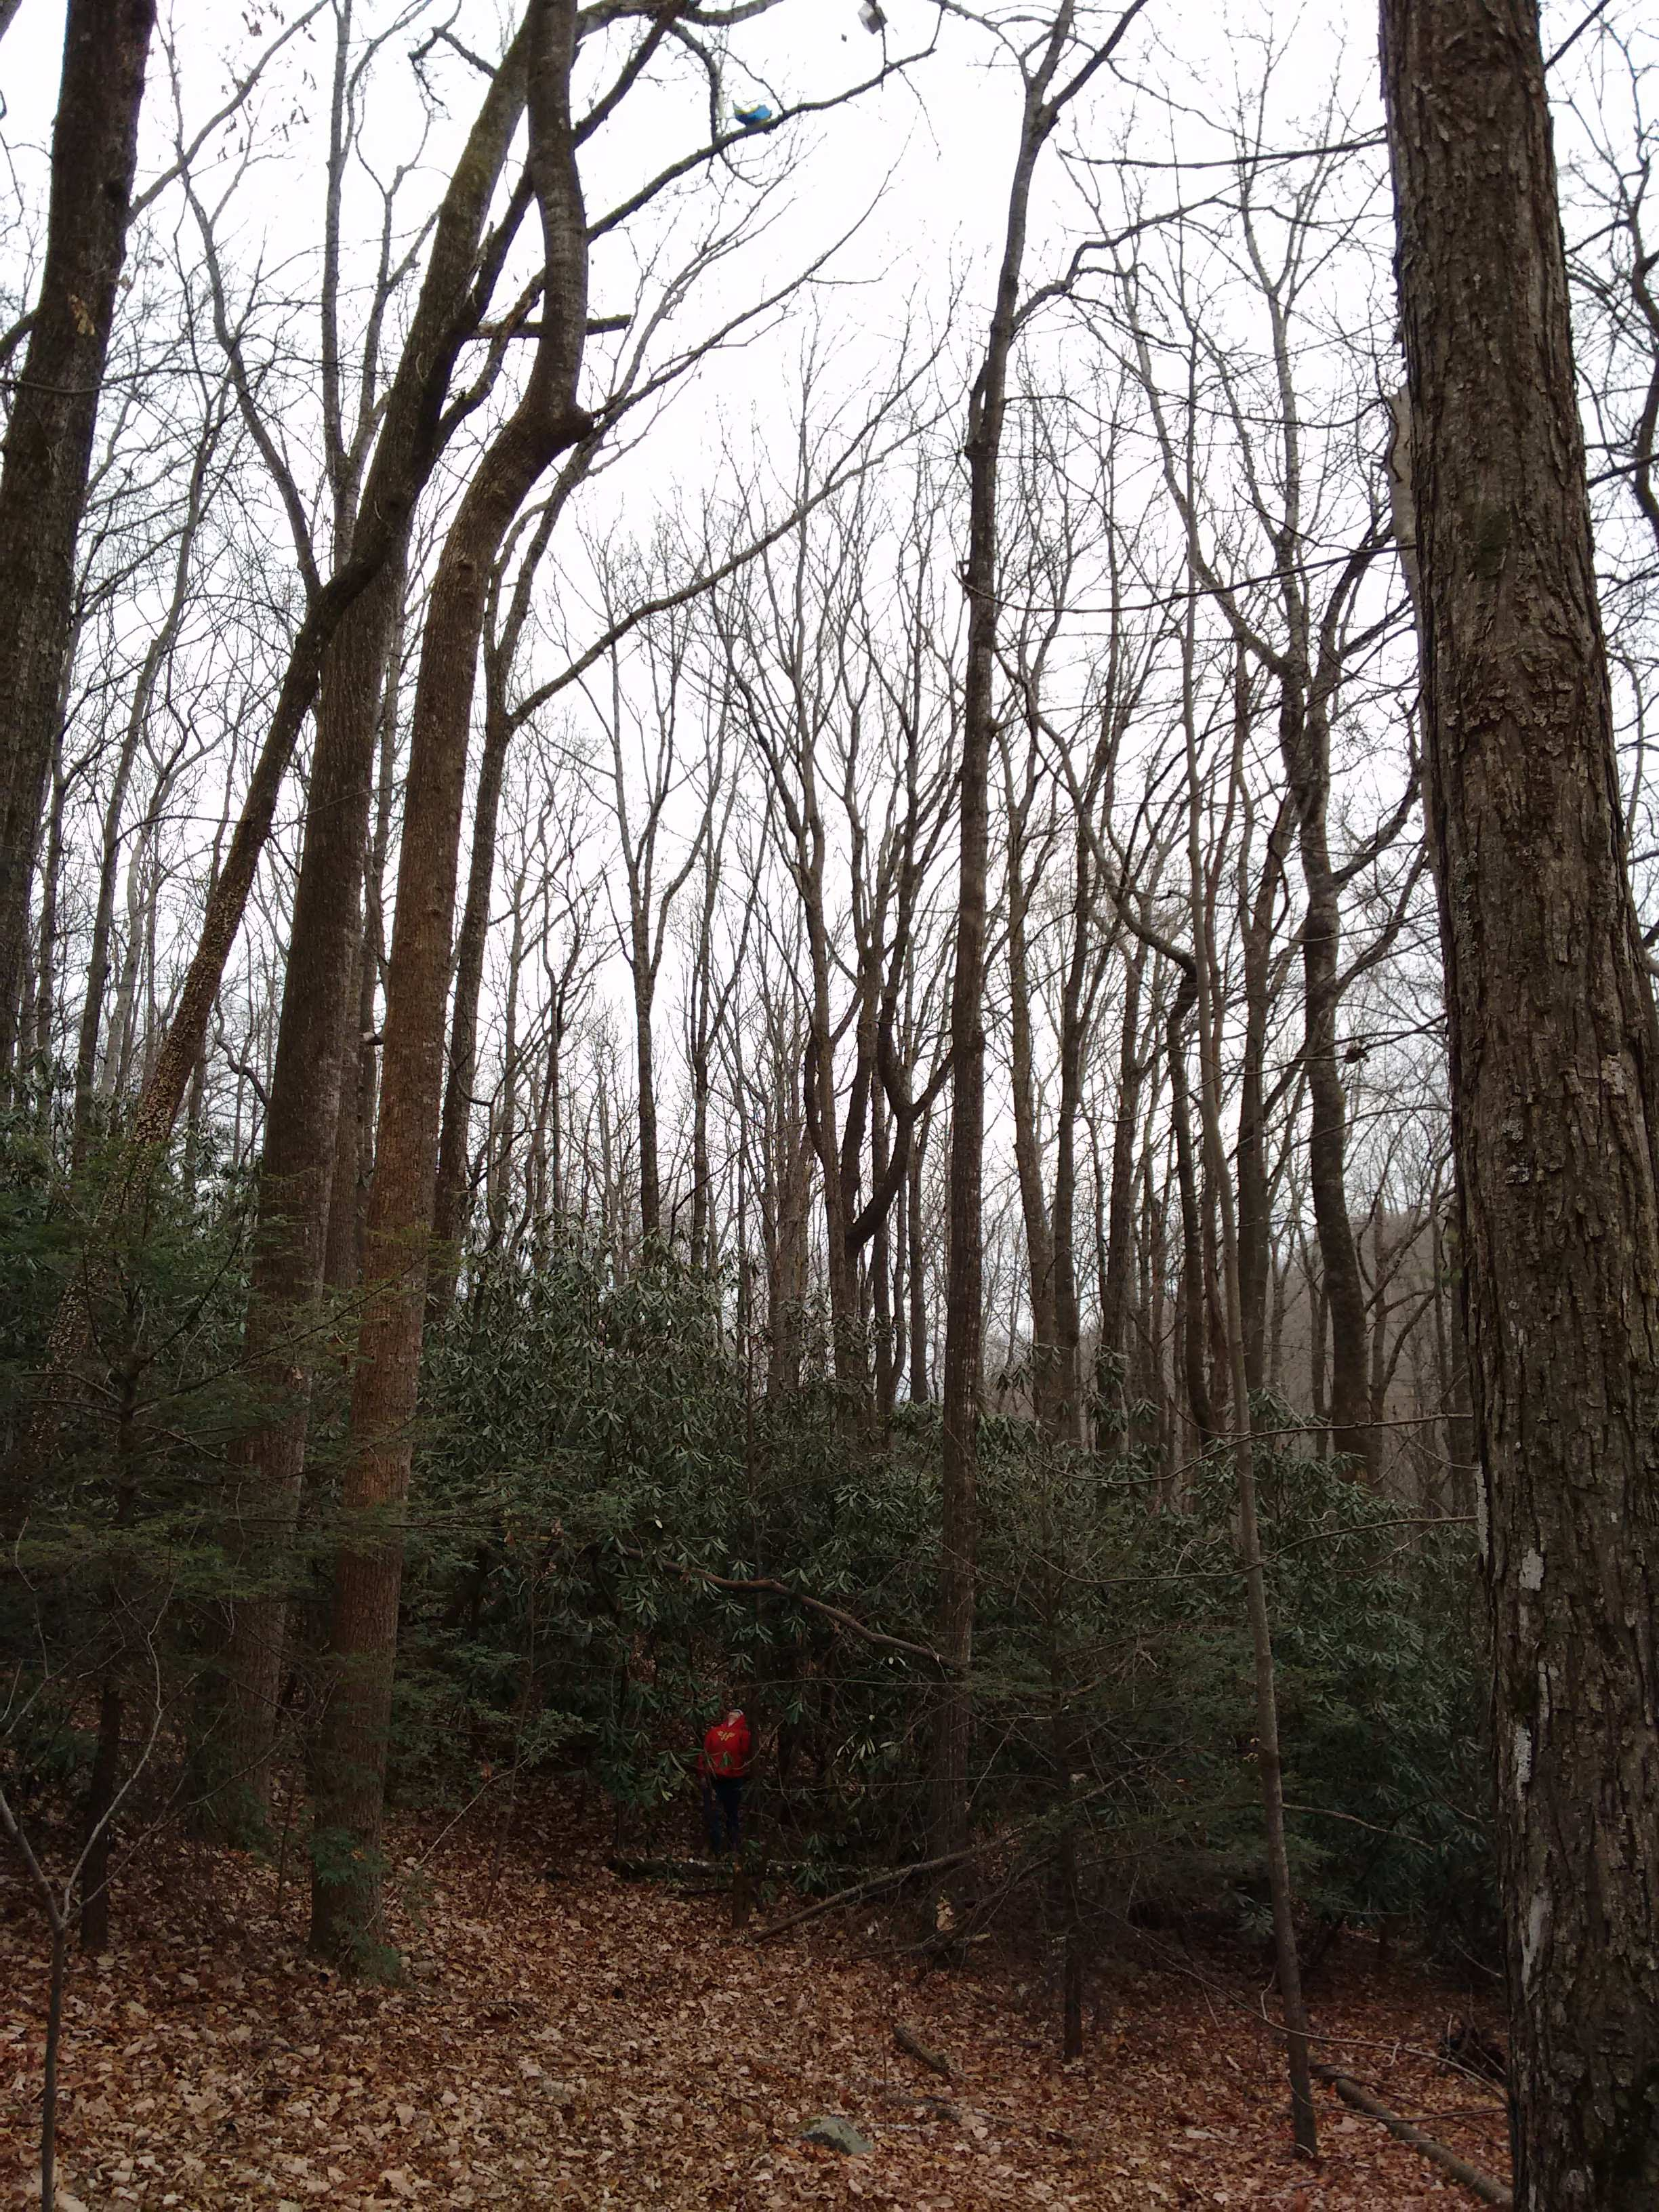
\includegraphics[height=0.75\textheight]{images/HabPi1_1}
        \caption{HabPi 1 in Tree}
    \end{figure}
\end{frame}

\section{HabPi}

\begin{frame}{Parts List}
\begin{table}
    \begin{center}
    \begin{tabular}{l|r}
        {\bf Item} & {\bf Approximate Cost}\\
        \hline
        Raspberry PI 3 Model B. & \$35.00\\
        Sense HAT & \$30.00\\
        Raspberry Pi Camera V2& \$30.00\\
        32GB Micro SD Card & \$15.00\\
        3 $\times$ DS18B20 Digital Thermometers & \$9.00\\
        4.7k$\Omega$ 1/4 W Resistor & \$0.10\\
        30 Row self-adhesive breadboard & \$5.00\\
        4400 mAh USB Battery (Cell Phone Charger) & \$10.00\\ 
        20 pack of Male/Female Jumper Wires & \$3.00\\
        300mm Ribbon Cable for Pi Camera & \$2.00\\
        \hline
        {\bf Total} & {\bf\$139.10} \\
    \end{tabular}
    \caption{Parts List}
    \label{tab:parts}
    \end{center}
\end{table}
\end{frame}

\begin{frame}{Sense HAT Sensor Limits}
\begin{itemize}
    \item Two Digital Thermometers ($-40 \celsius$ to $+120 \celsius$)
    \cite{HTS221} and ($-30 \celsius$ to $+105 \celsius$)\cite{LPS25H}
    \item Barometric Pressure Sensor (260 to 1260 hPa) ~\cite{LPS25H}
    \item Relative Humidity Sensor ($0\%$ to $100\%$)~\cite{HTS221}
    \item 3-Axis Magnetometer ($\pm 16$ gauss)~\cite{LSM9DS1}
    \item 3-Axis Gyroscope ($\pm 2000$ dps)~\cite{LSM9DS1}
    \item 3-Axis Accelerometer ($\pm 16$g)~\cite{LSM9DS1}
    \item Joystick for Input
    \item RGB LED Array for Output
\end{itemize}
\end{frame}

\begin{frame}{Wiring the Sense HAT}
\begin{figure}
    \centering
    \begin{subfigure}{.45\textwidth}
        \centering
        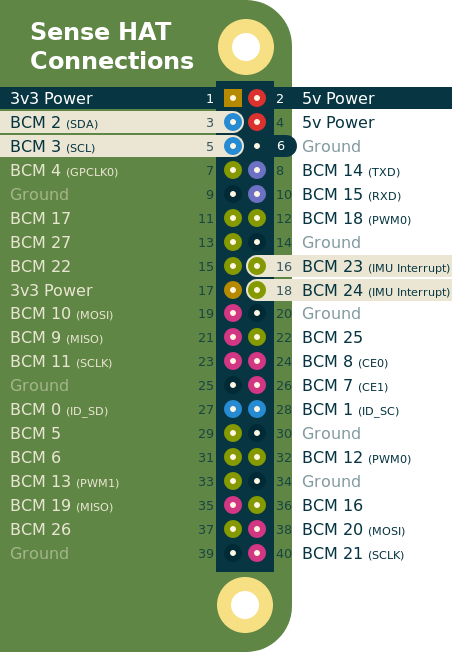
\includegraphics[height=0.7\textheight]{images/rpi-sensehat}
        \caption{Minimal Raspberry Pi Sense HAT
        Connections~\cite{pinout}}
        \label{fig:pinout}
    \end{subfigure}
    \begin{subfigure}{.45\textwidth}
        \centering
        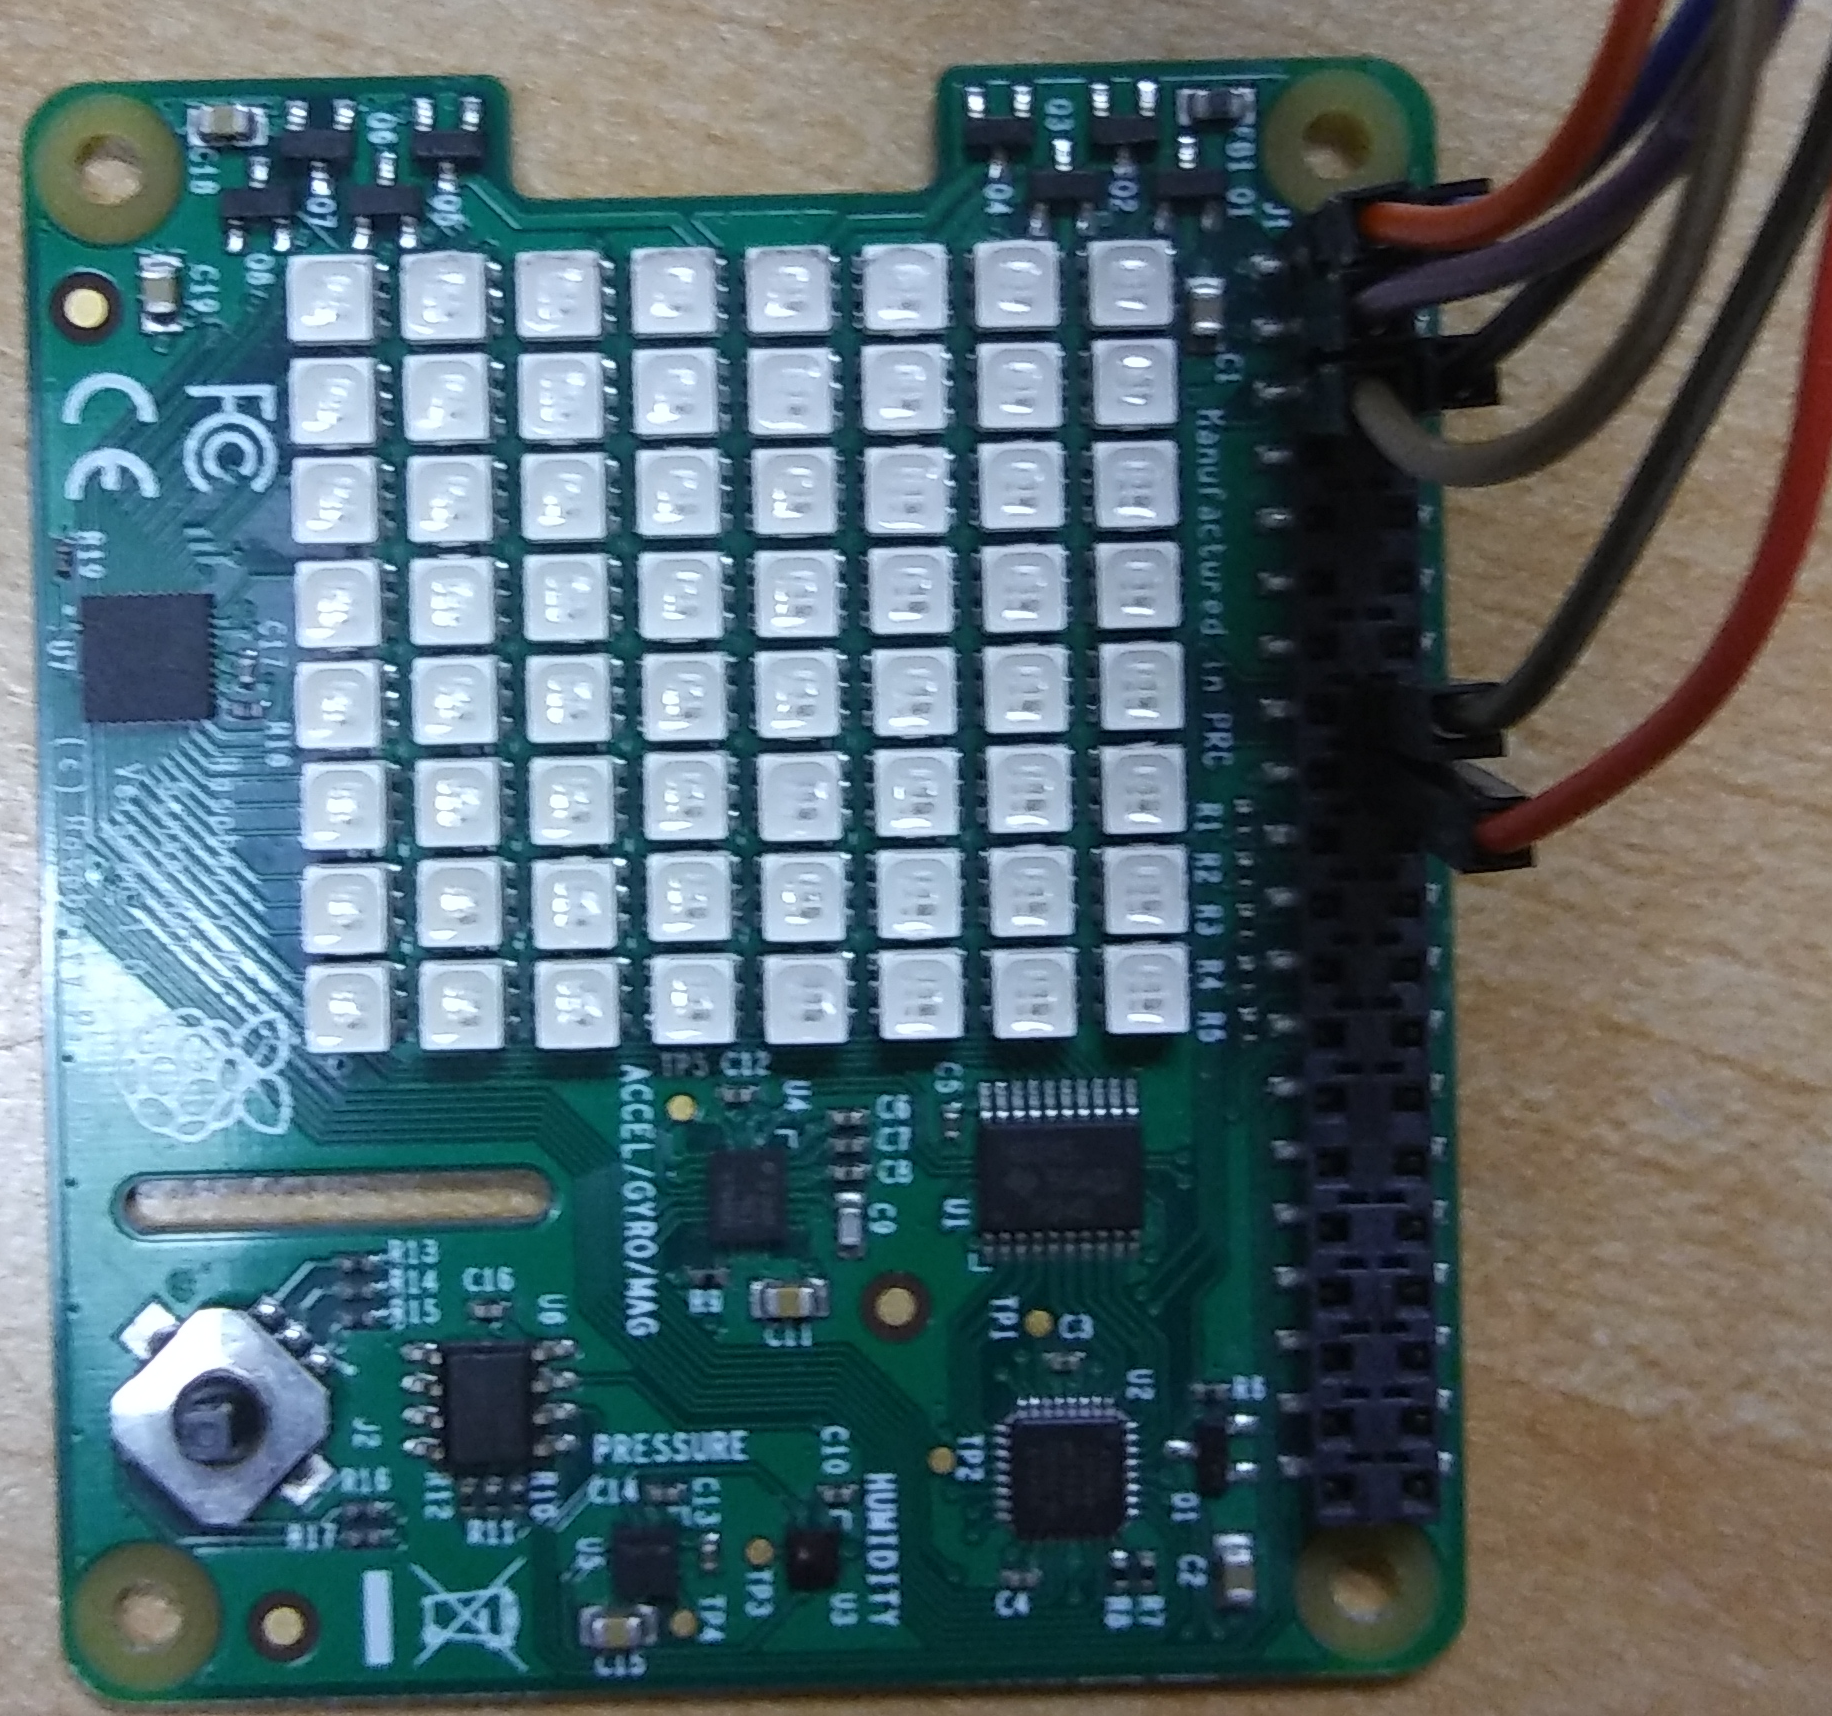
\includegraphics[width=\textwidth]{images/sensehat}
        \caption{Sense Hat Connections}
        \label{fig:hat}
    \end{subfigure}
    \caption{Wiring the Sense Hat}
    \label{fig:hatwiring}
\end{figure}
\end{frame}

\begin{frame}{1-Wire Bus}
\begin{figure}
    \centering
    
\includegraphics[height=0.6\textheight]{images/ds18b20-circuit}
    \caption{DS18B20 1-Wire Circuit}
    \label{fig:circuit}
\end{figure}
\end{frame}

\begin{frame}{Complete Interior}
\begin{figure}
	\centering
        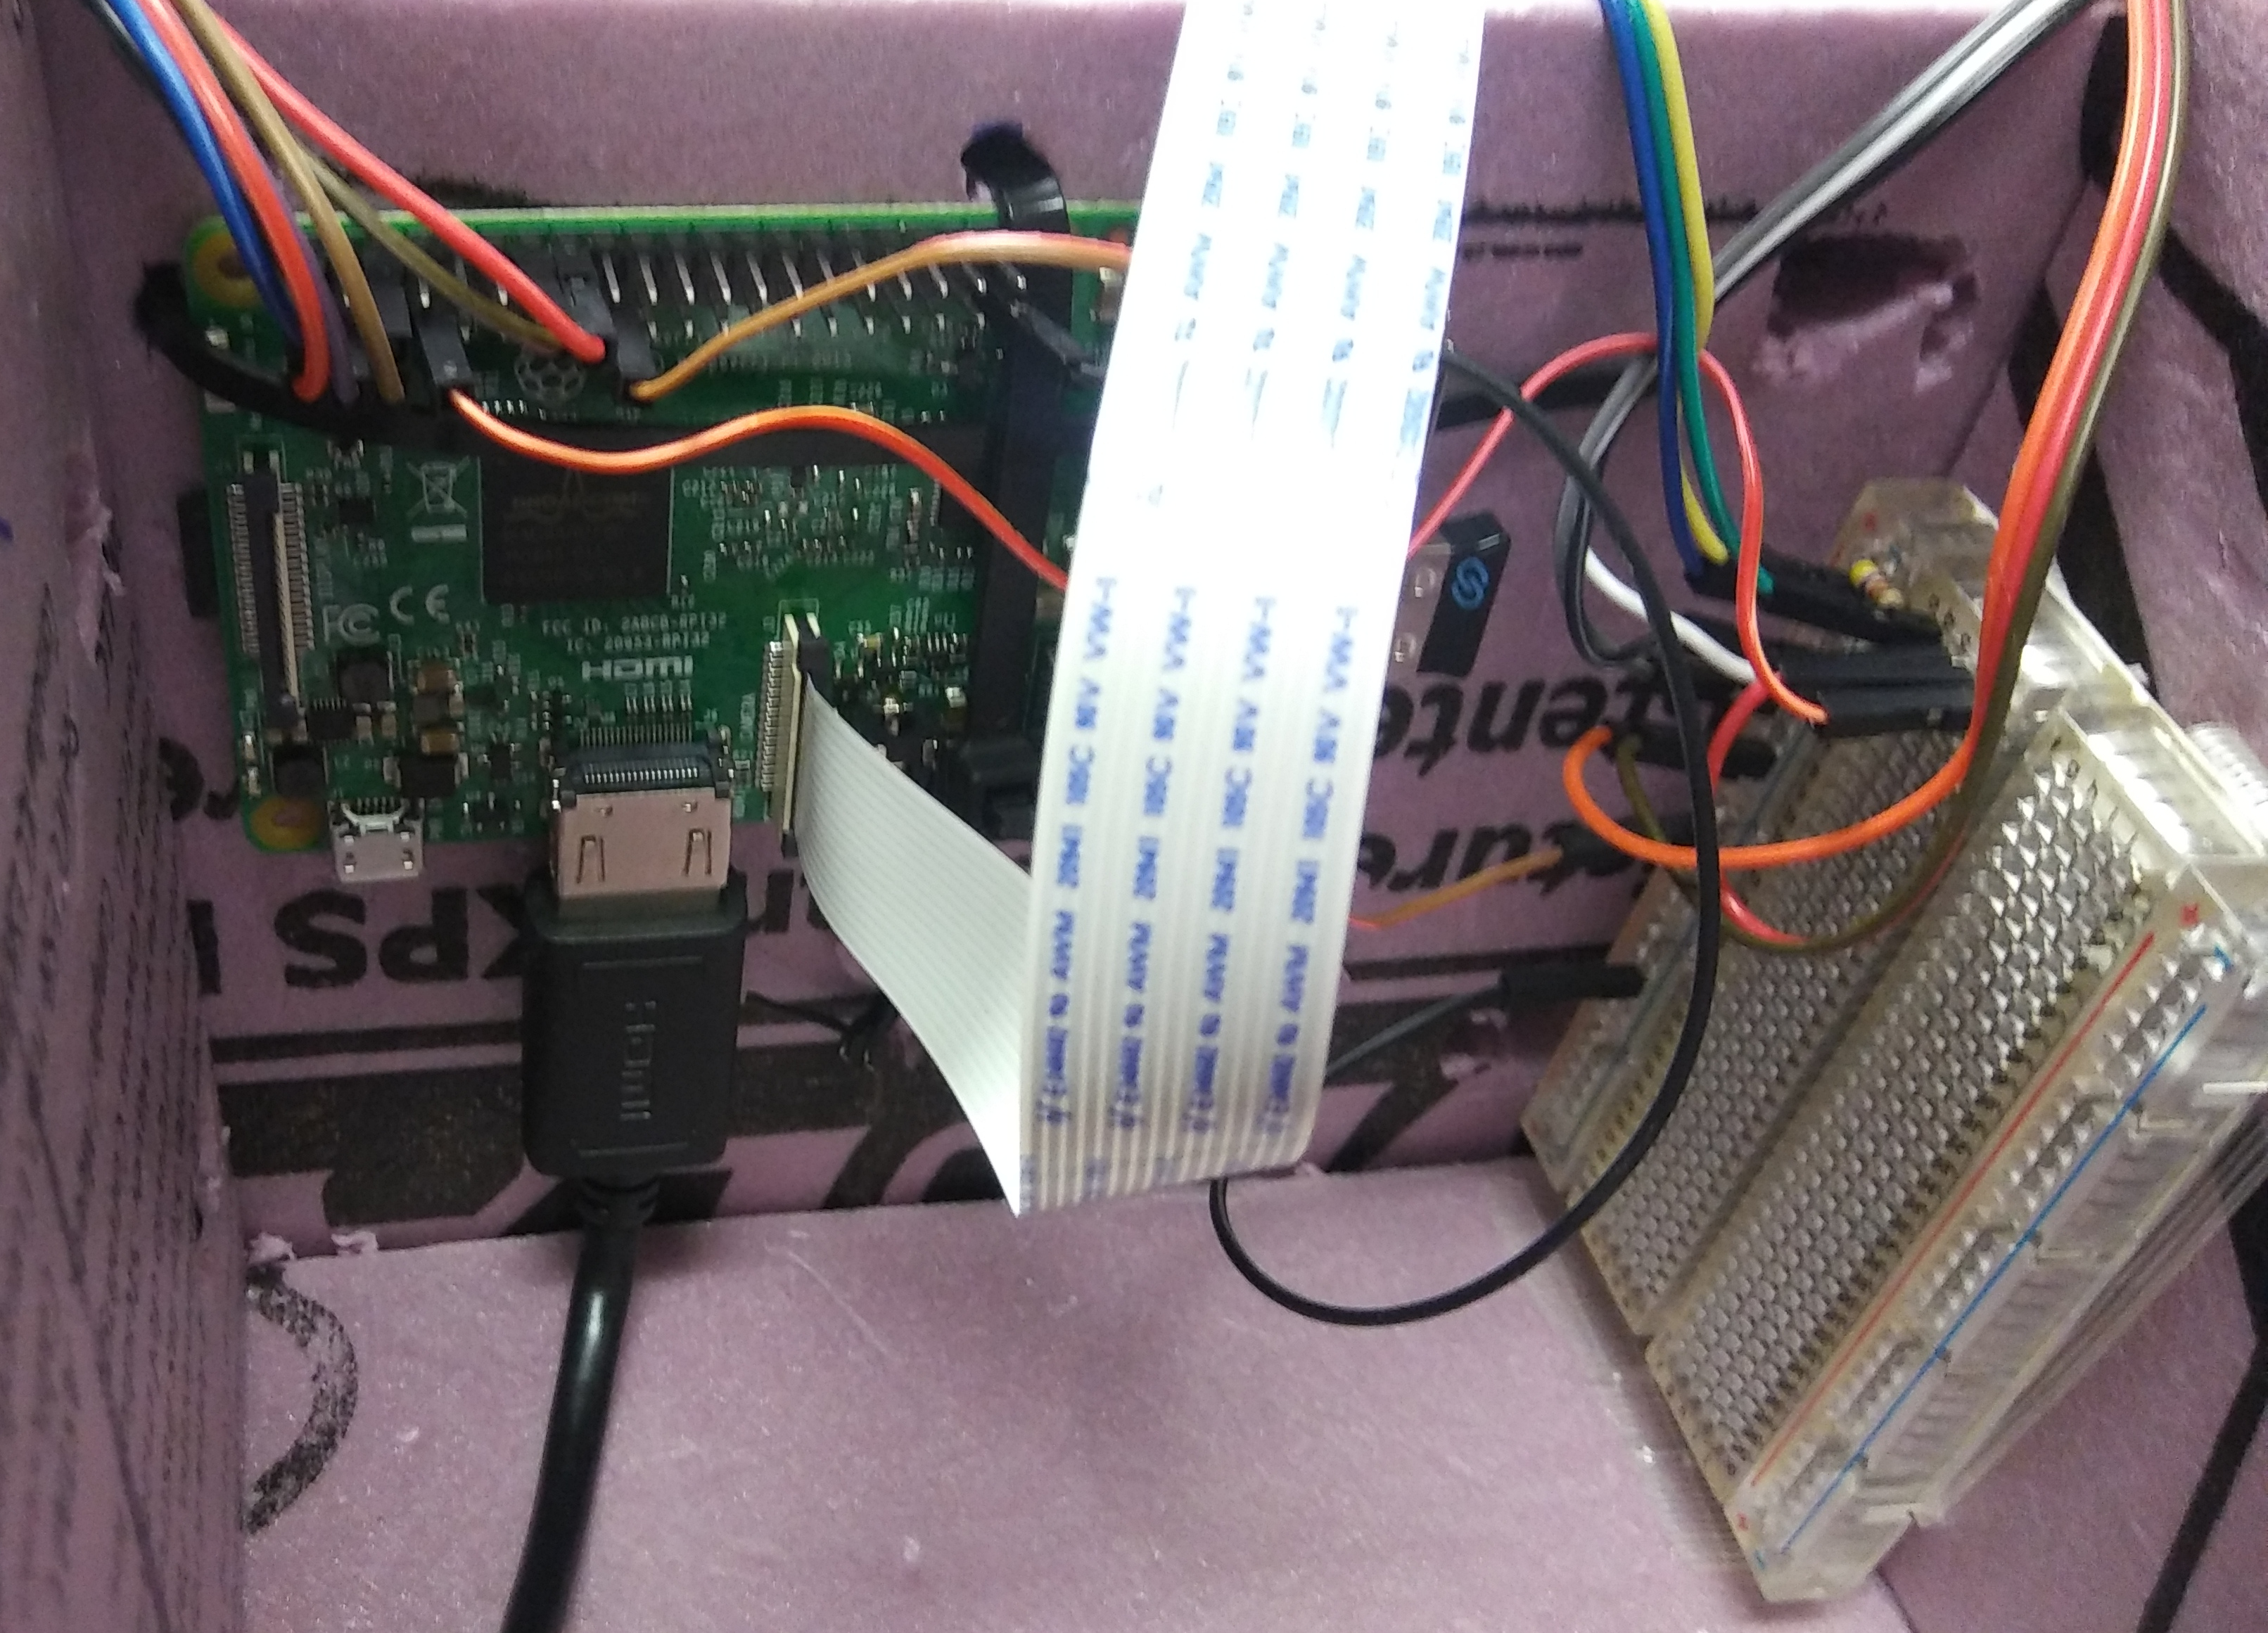
\includegraphics[height=0.75\textheight]{images/interior}
	\caption{HabPi Interior}
\end{figure}
\end{frame}

\begin{frame}{HabPi Software}
	\begin{itemize}
	\item Creates an access point with a configurable network for wireless data access
	\item Provides a simple user interface using the SenseHat
	\item Creates a time-labeled data directory under {\tt /home/pi/habpi/data}
	\item Executes experiments contained in {\tt /home/pi/habpi/experiments}
	\end{itemize}
\end{frame}

\begin{frame}{Raw Temperature Data}
	\begin{figure}
		\centering
		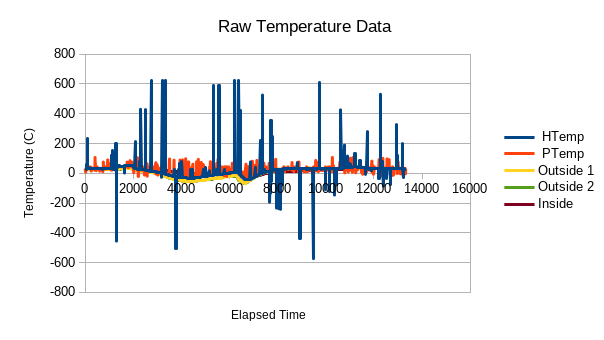
\includegraphics[height=0.75\textheight]{images/rawtemp}
		\caption{Raw Temperature Data}
	\end{figure}
\end{frame}

\begin{frame}{1-Wire Data}
	\begin{figure}
		\centering
		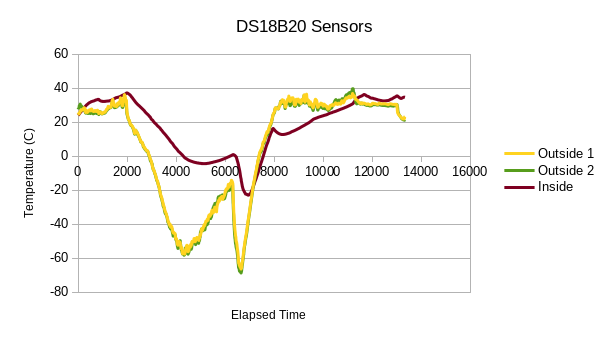
\includegraphics[height=0.75\textheight]{images/ds18b20-data}
		\caption{DS18B20 Temperature Data}
	\end{figure}
\end{frame}

\begin{frame}{Smoothed Temperature Data}
	\begin{figure}
		\centering
		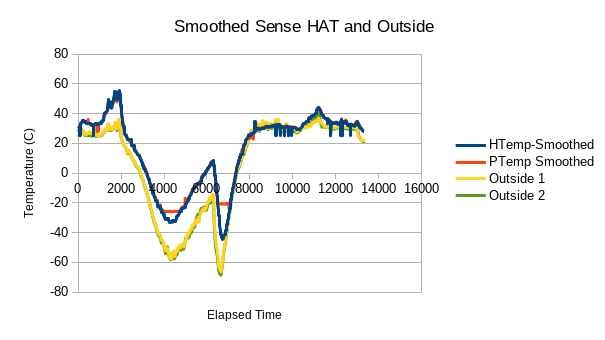
\includegraphics[height=0.75\textheight]{images/smoothtemp}
		\caption{Smoothed Temperature Data}
	\end{figure}
\end{frame}

\section{HabPi Flights}

\begin{frame}[t]{HabPi 2 - March 19, 2017}
    \begin{columns}[t]
        \column{0.5\textwidth}
        \begin{itemize}
            \item Reference HabPi device built by Robert Lowe
            \item Released from Russell Springs Kentucky
            \item Reached an Altitude of 42,000 Meters
            \item Recovered near New River, TN
        \end{itemize}

        \column{0.5\textwidth}
        \begin{figure}
            \centering
            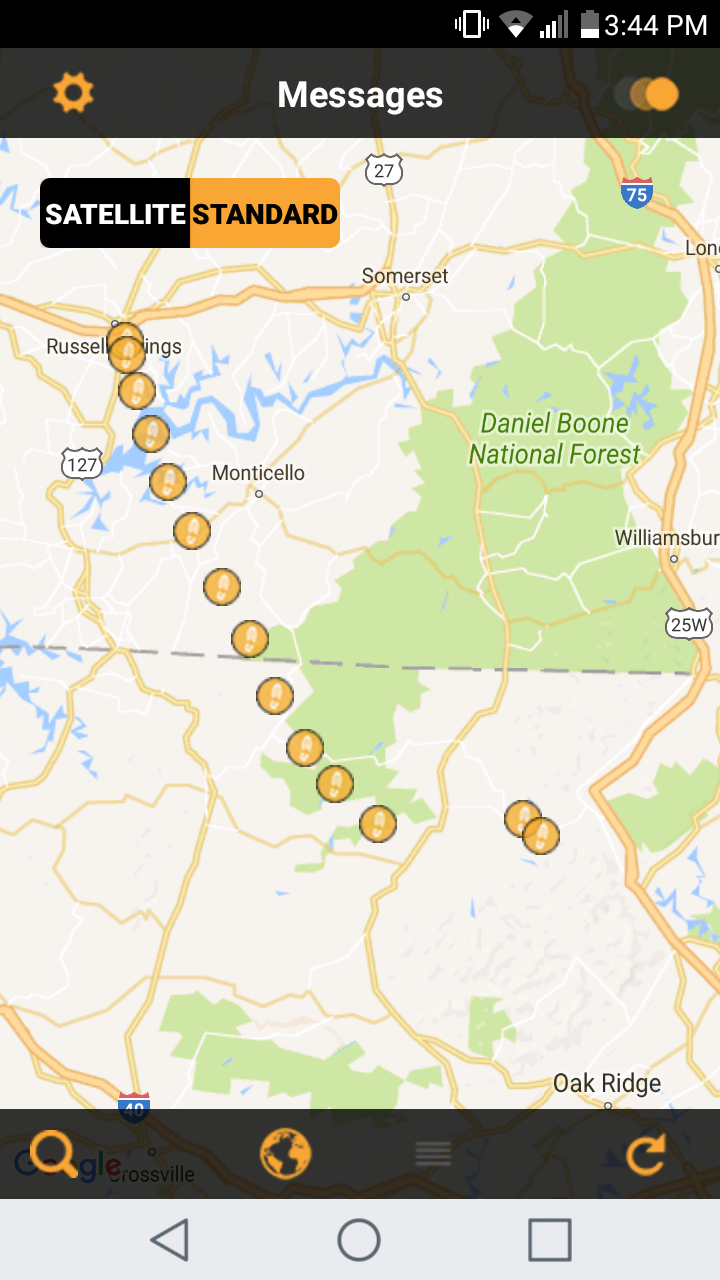
\includegraphics[height=0.6\textheight]{images/habpi2_track}
            \caption{\tiny HabPi 2 Spot Tracker}
        \end{figure}
    \end{columns}
\end{frame}

\begin{frame}{HabPi 2 - March 19, 2017}
    \begin{figure}
        \centering
        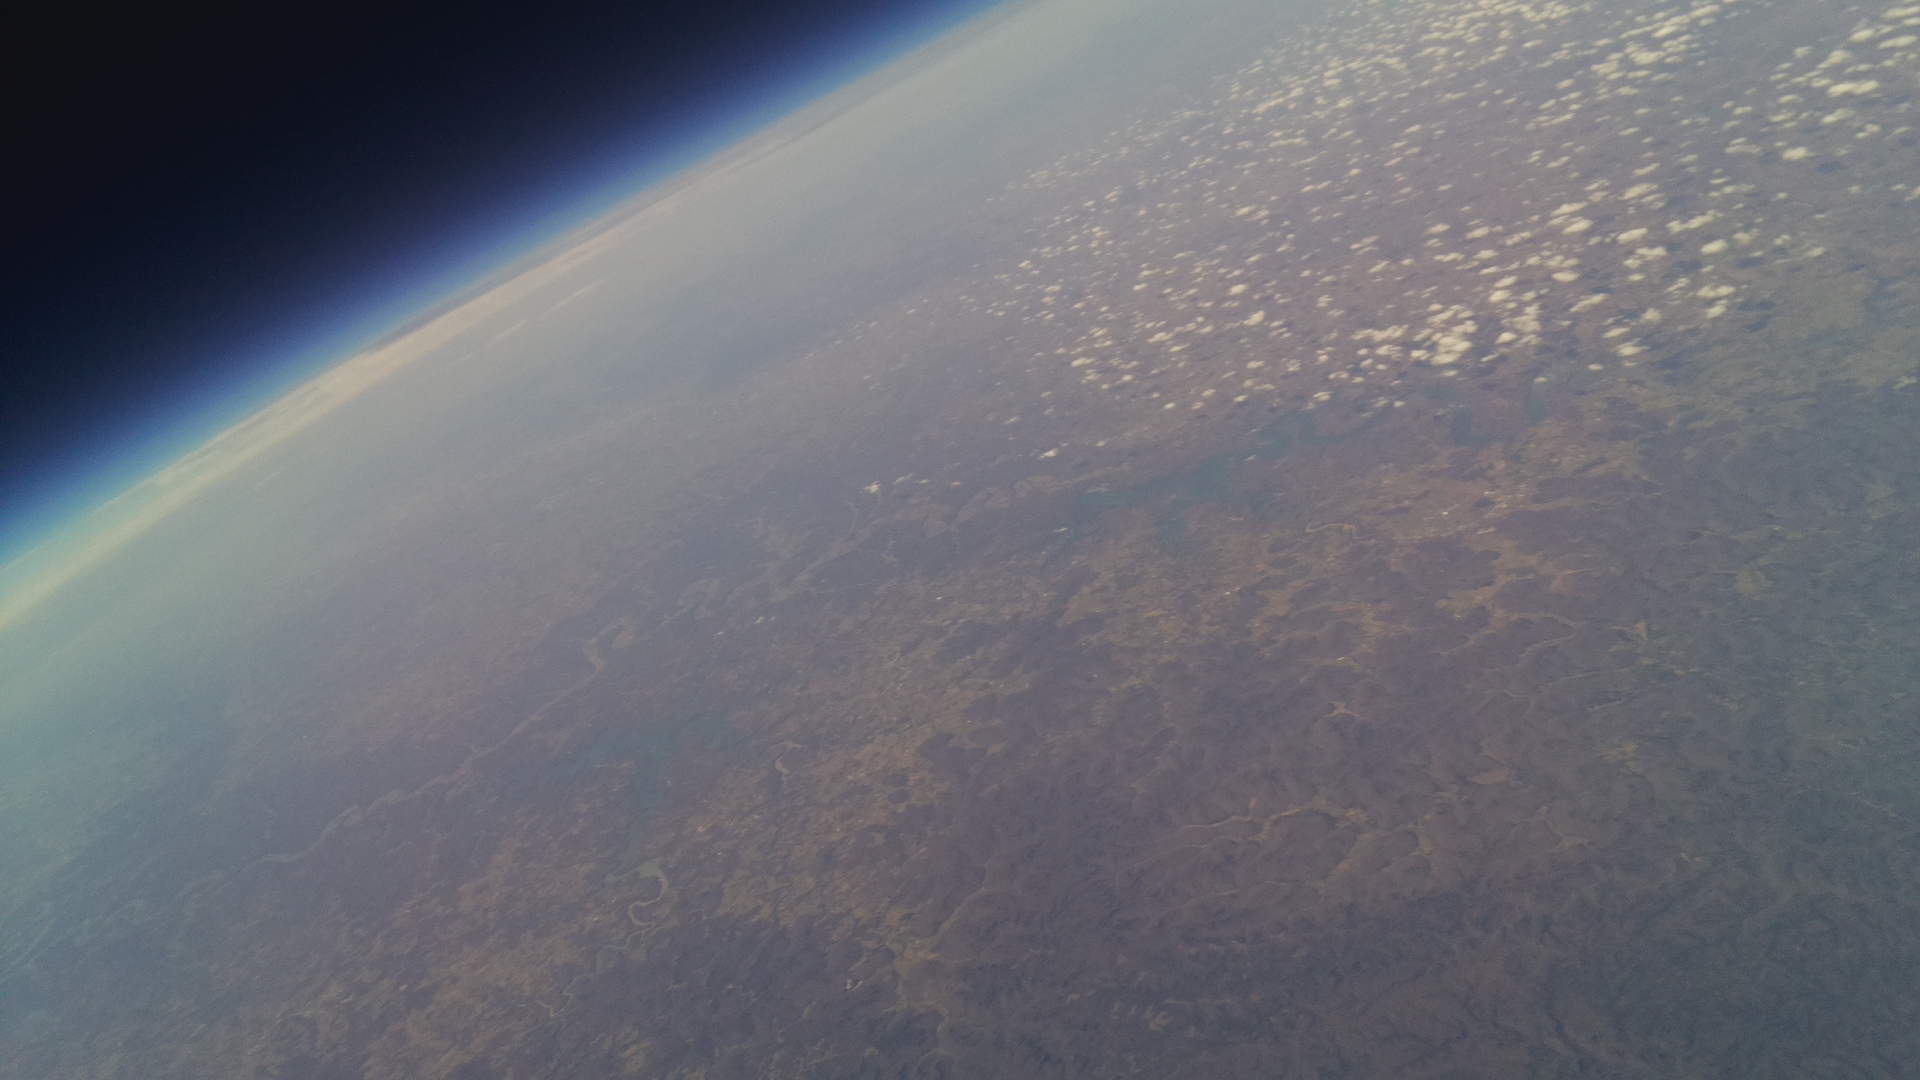
\includegraphics[width=\textwidth]{images/habpi2_1}
    \end{figure}
\end{frame}

\begin{frame}{HabPi 2 - March 19, 2017}
    \begin{figure}
        \centering
        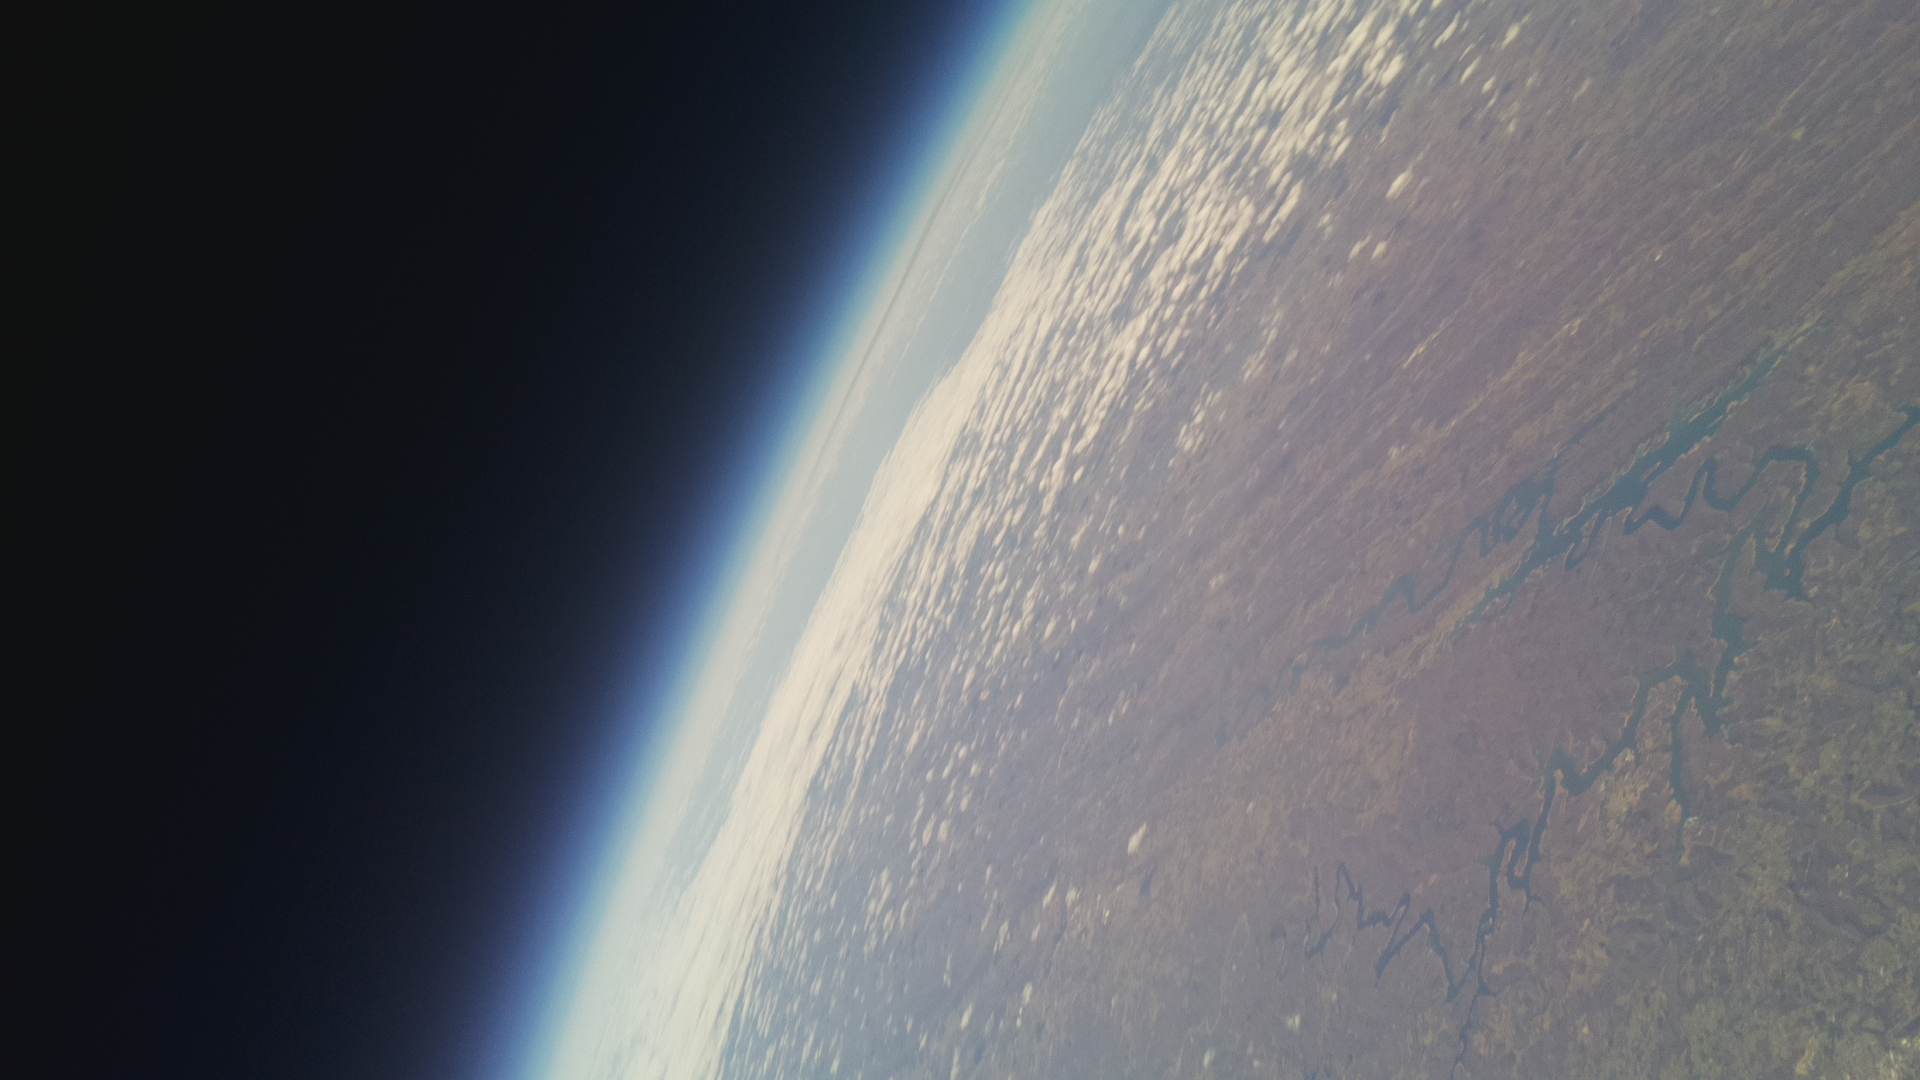
\includegraphics[width=\textwidth]{images/habpi2_2}
    \end{figure}
\end{frame}

\begin{frame}{HabPi 2 - March 19, 2017}
    \begin{figure}
        \centering
        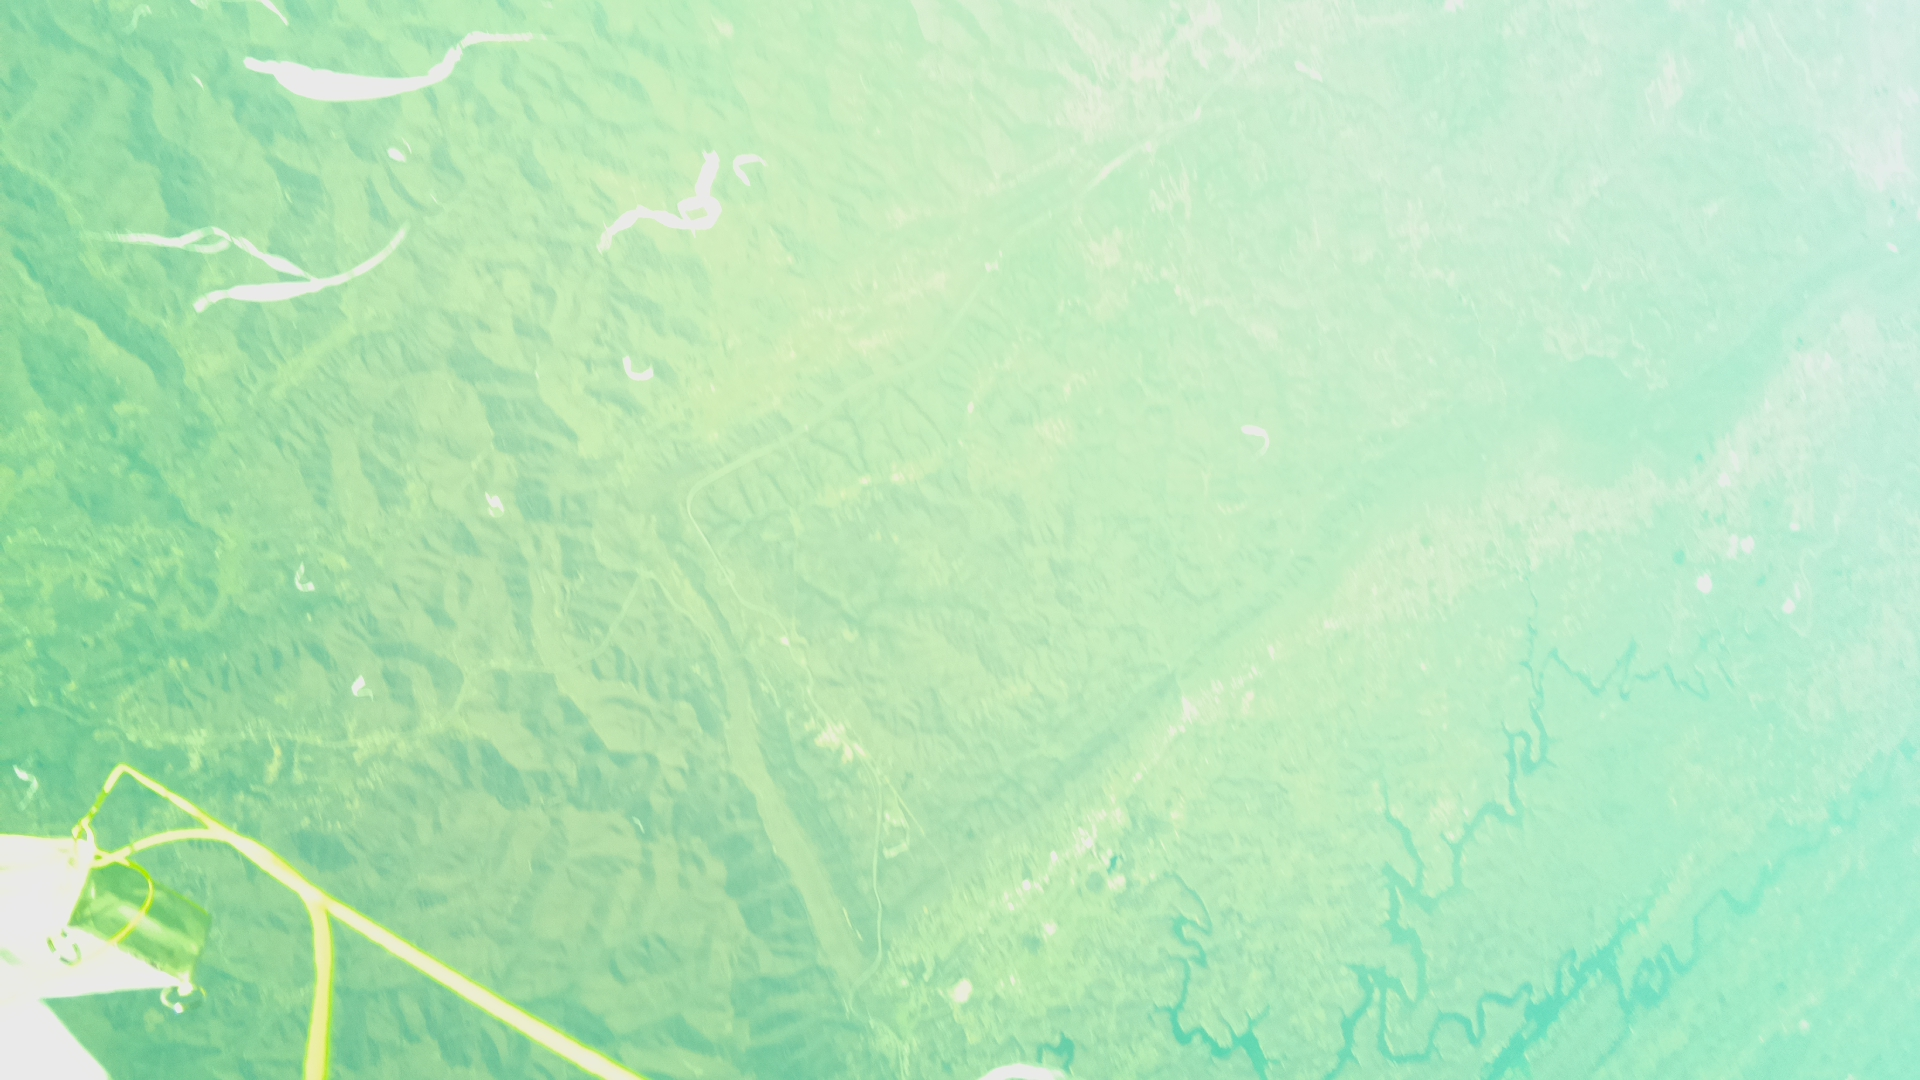
\includegraphics[width=\textwidth]{images/habpi2_3}
    \end{figure}
\end{frame}

\begin{frame}{HabPi 2 - March 19, 2017}
    \begin{figure}
        \centering
        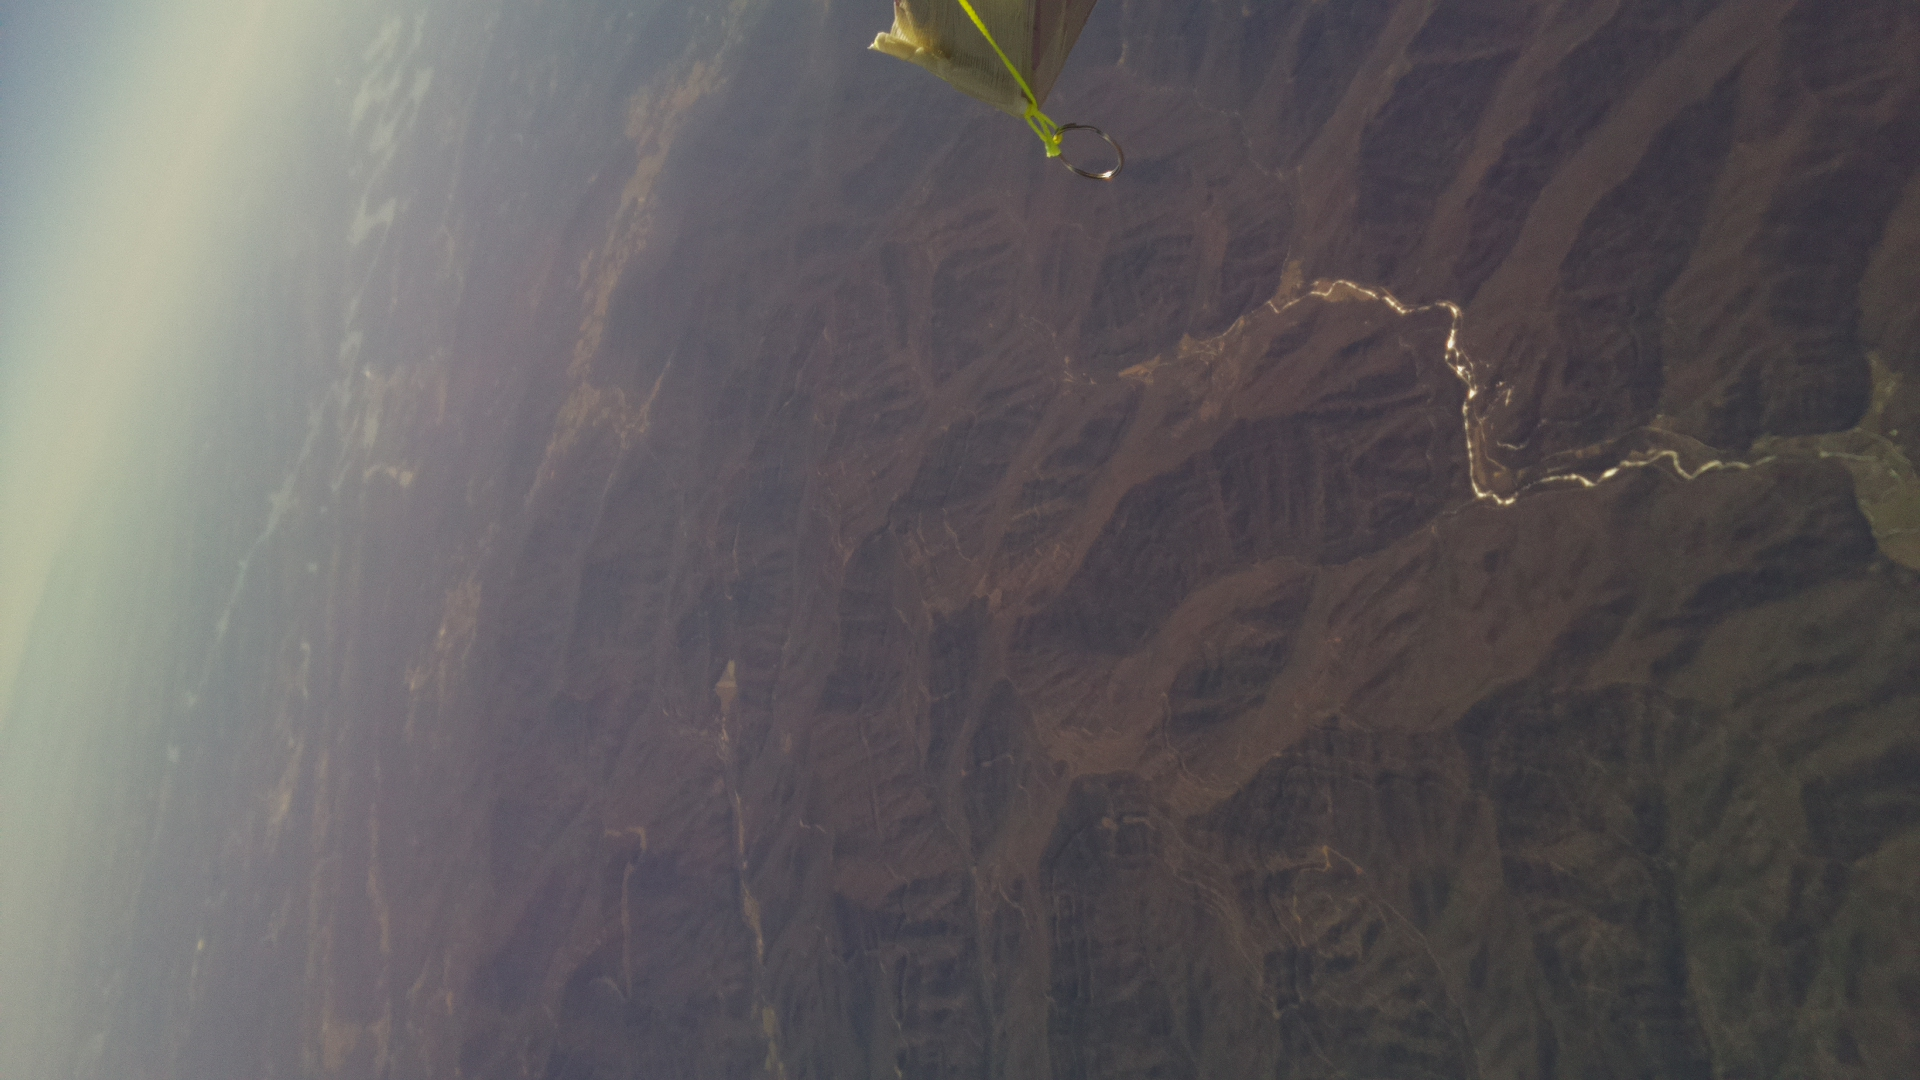
\includegraphics[width=\textwidth]{images/habpi2_4}
    \end{figure}
\end{frame}

\begin{frame}{HabPi 3 - May 13, 2017}
    \begin{columns}[t]
        \column{0.5\textwidth}
        \begin{itemize}
            \item 3 HabPi Payloads constructed by students from Concord Christian School
            \item 1 HabPi Payload constructed by BSA Troop 255
	    \item Released in Sunbright TN
            \item Reached an Altitude of 27,000 Meters 
	    \item Flew through restricted air space at low altitude
        \end{itemize}

        \column{0.5\textwidth}
        \begin{figure}
            \centering
            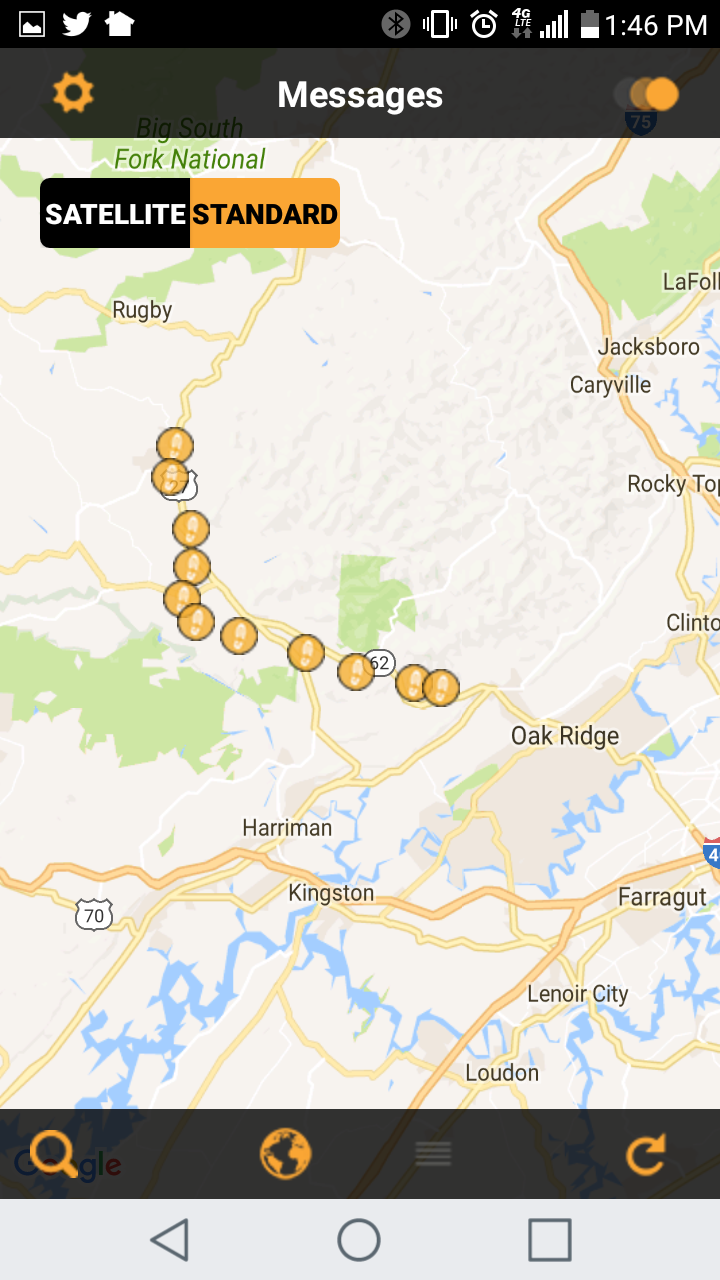
\includegraphics[height=0.6\textheight]{images/habpi3_track}
            \caption{\tiny HabPi 3 Spot Tracker}
        \end{figure}
    \end{columns}
\end{frame}

\begin{frame}{HabPi 3 - May 13, 2017}
    \begin{figure}
        \centering
        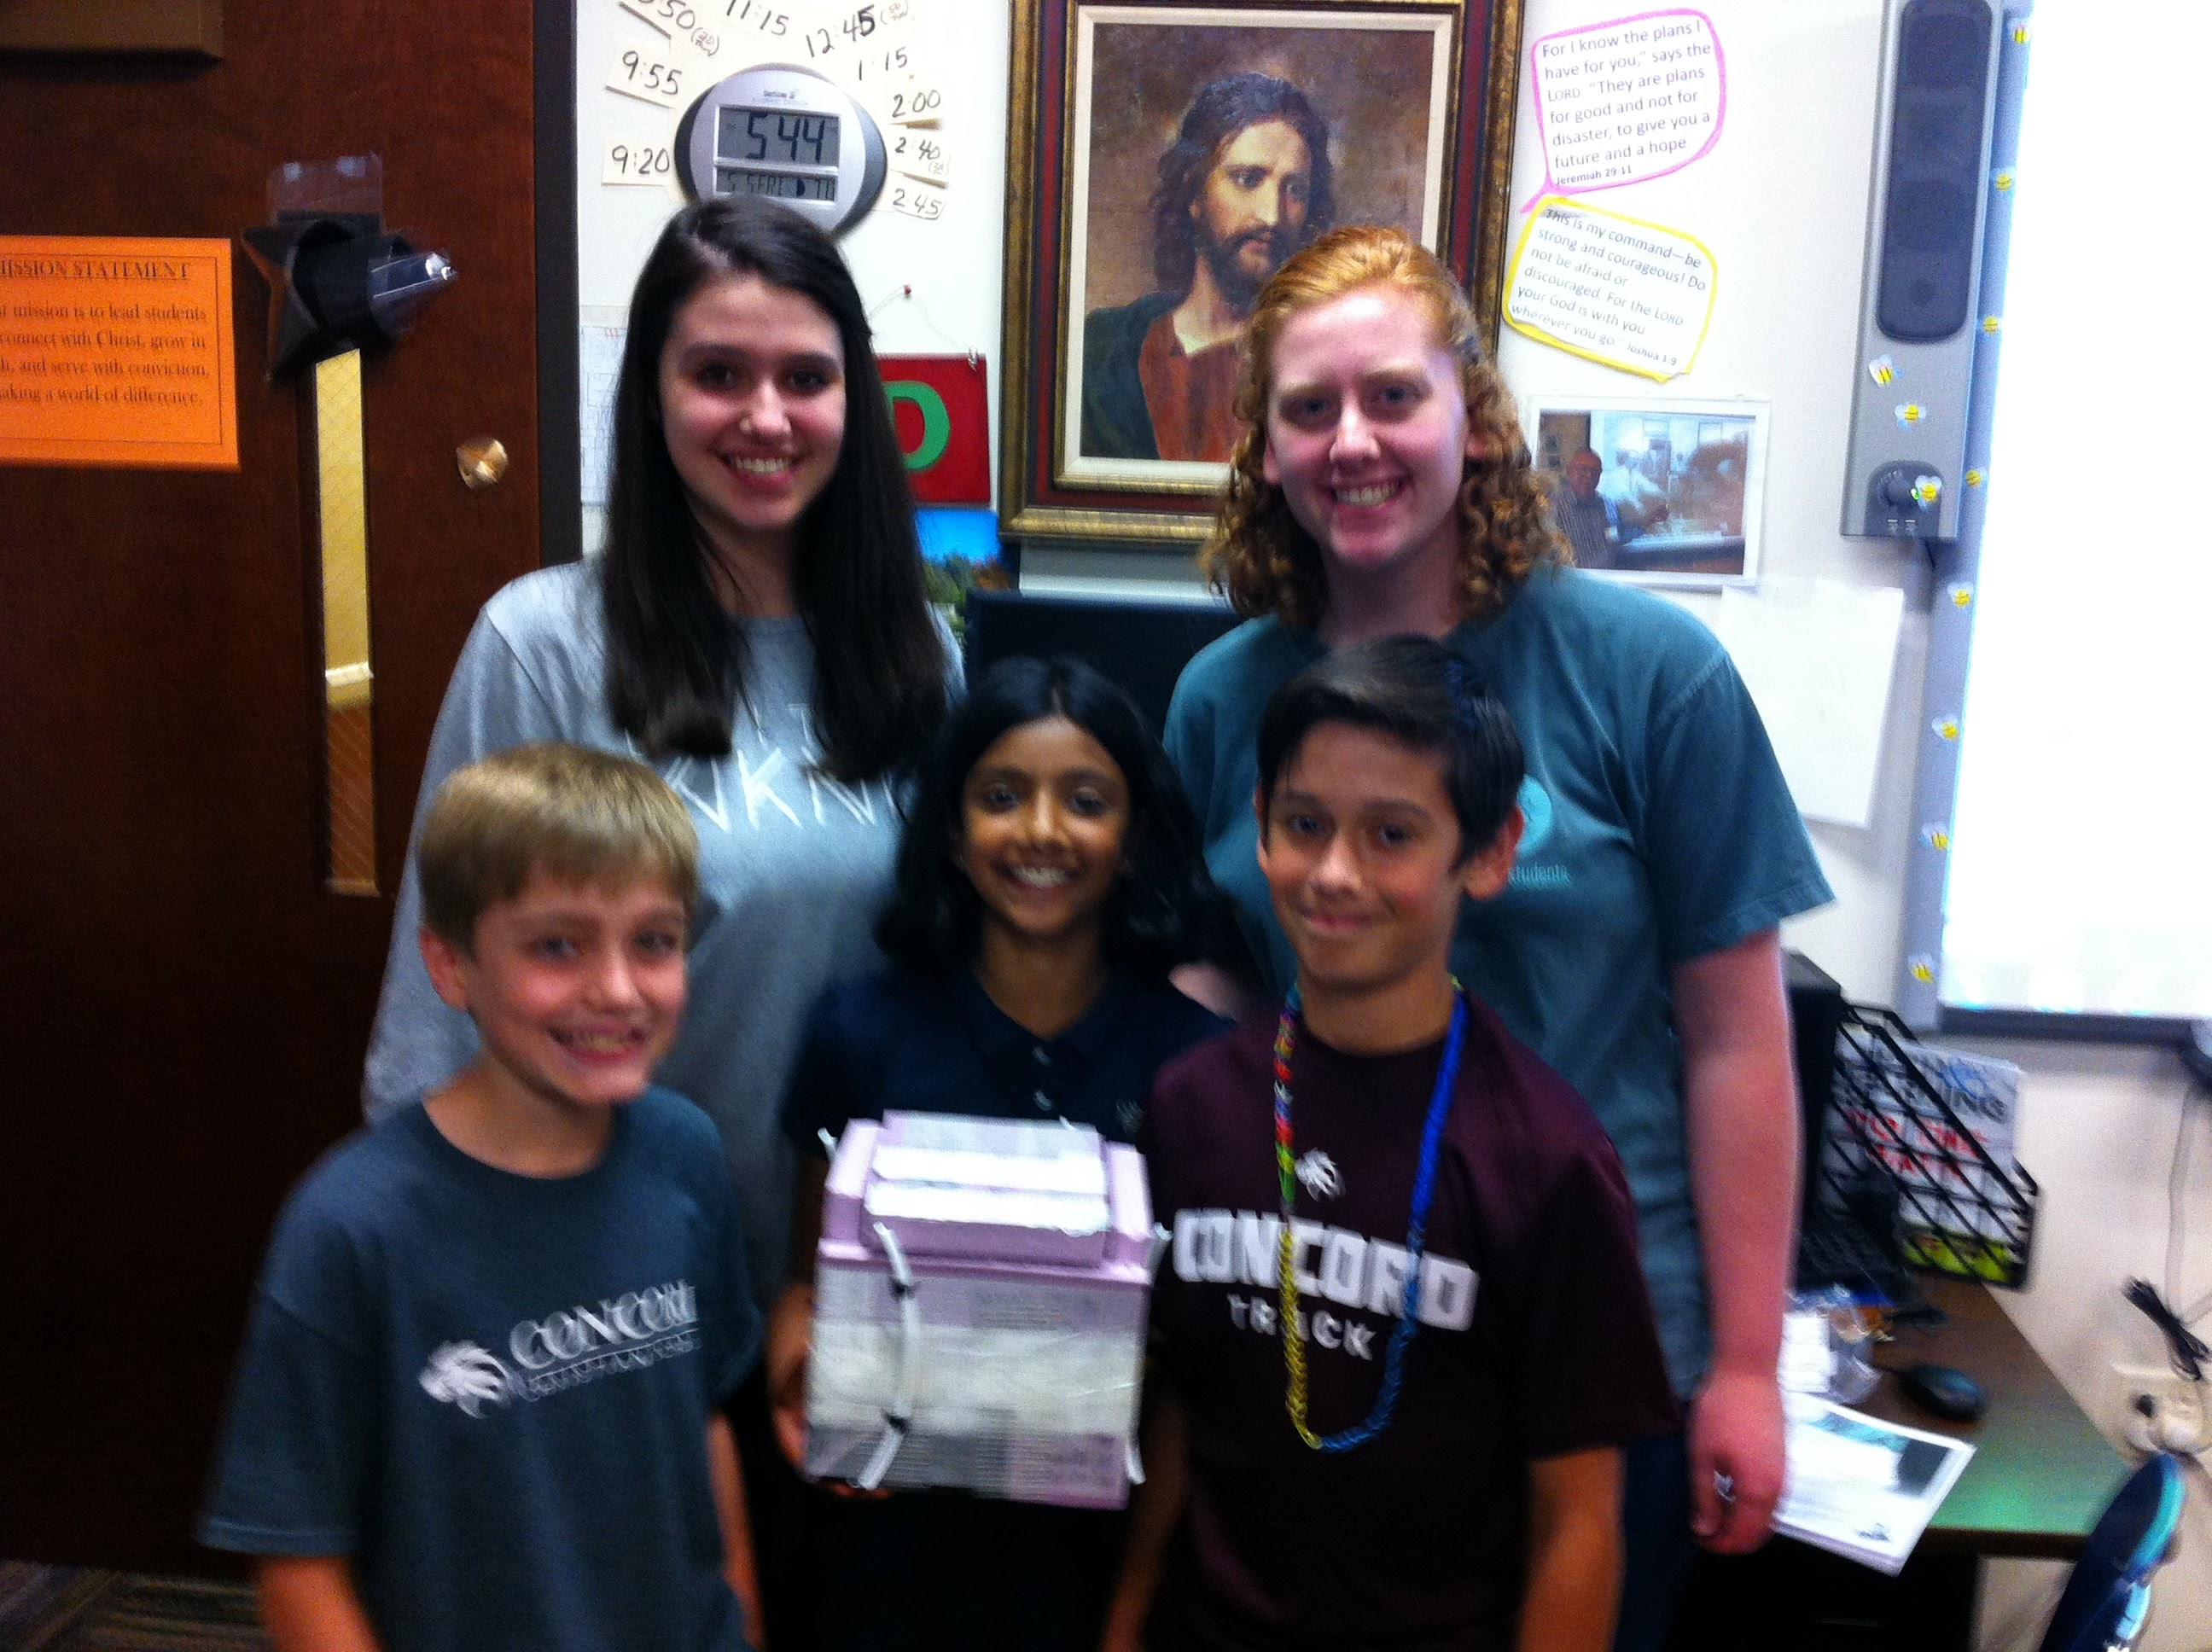
\includegraphics[height=0.7\textheight]{images/CCS_Payload}
    \end{figure}
\end{frame}

\begin{frame}{HabPi 3 - May 13, 2017}
    \begin{figure}
        \centering
        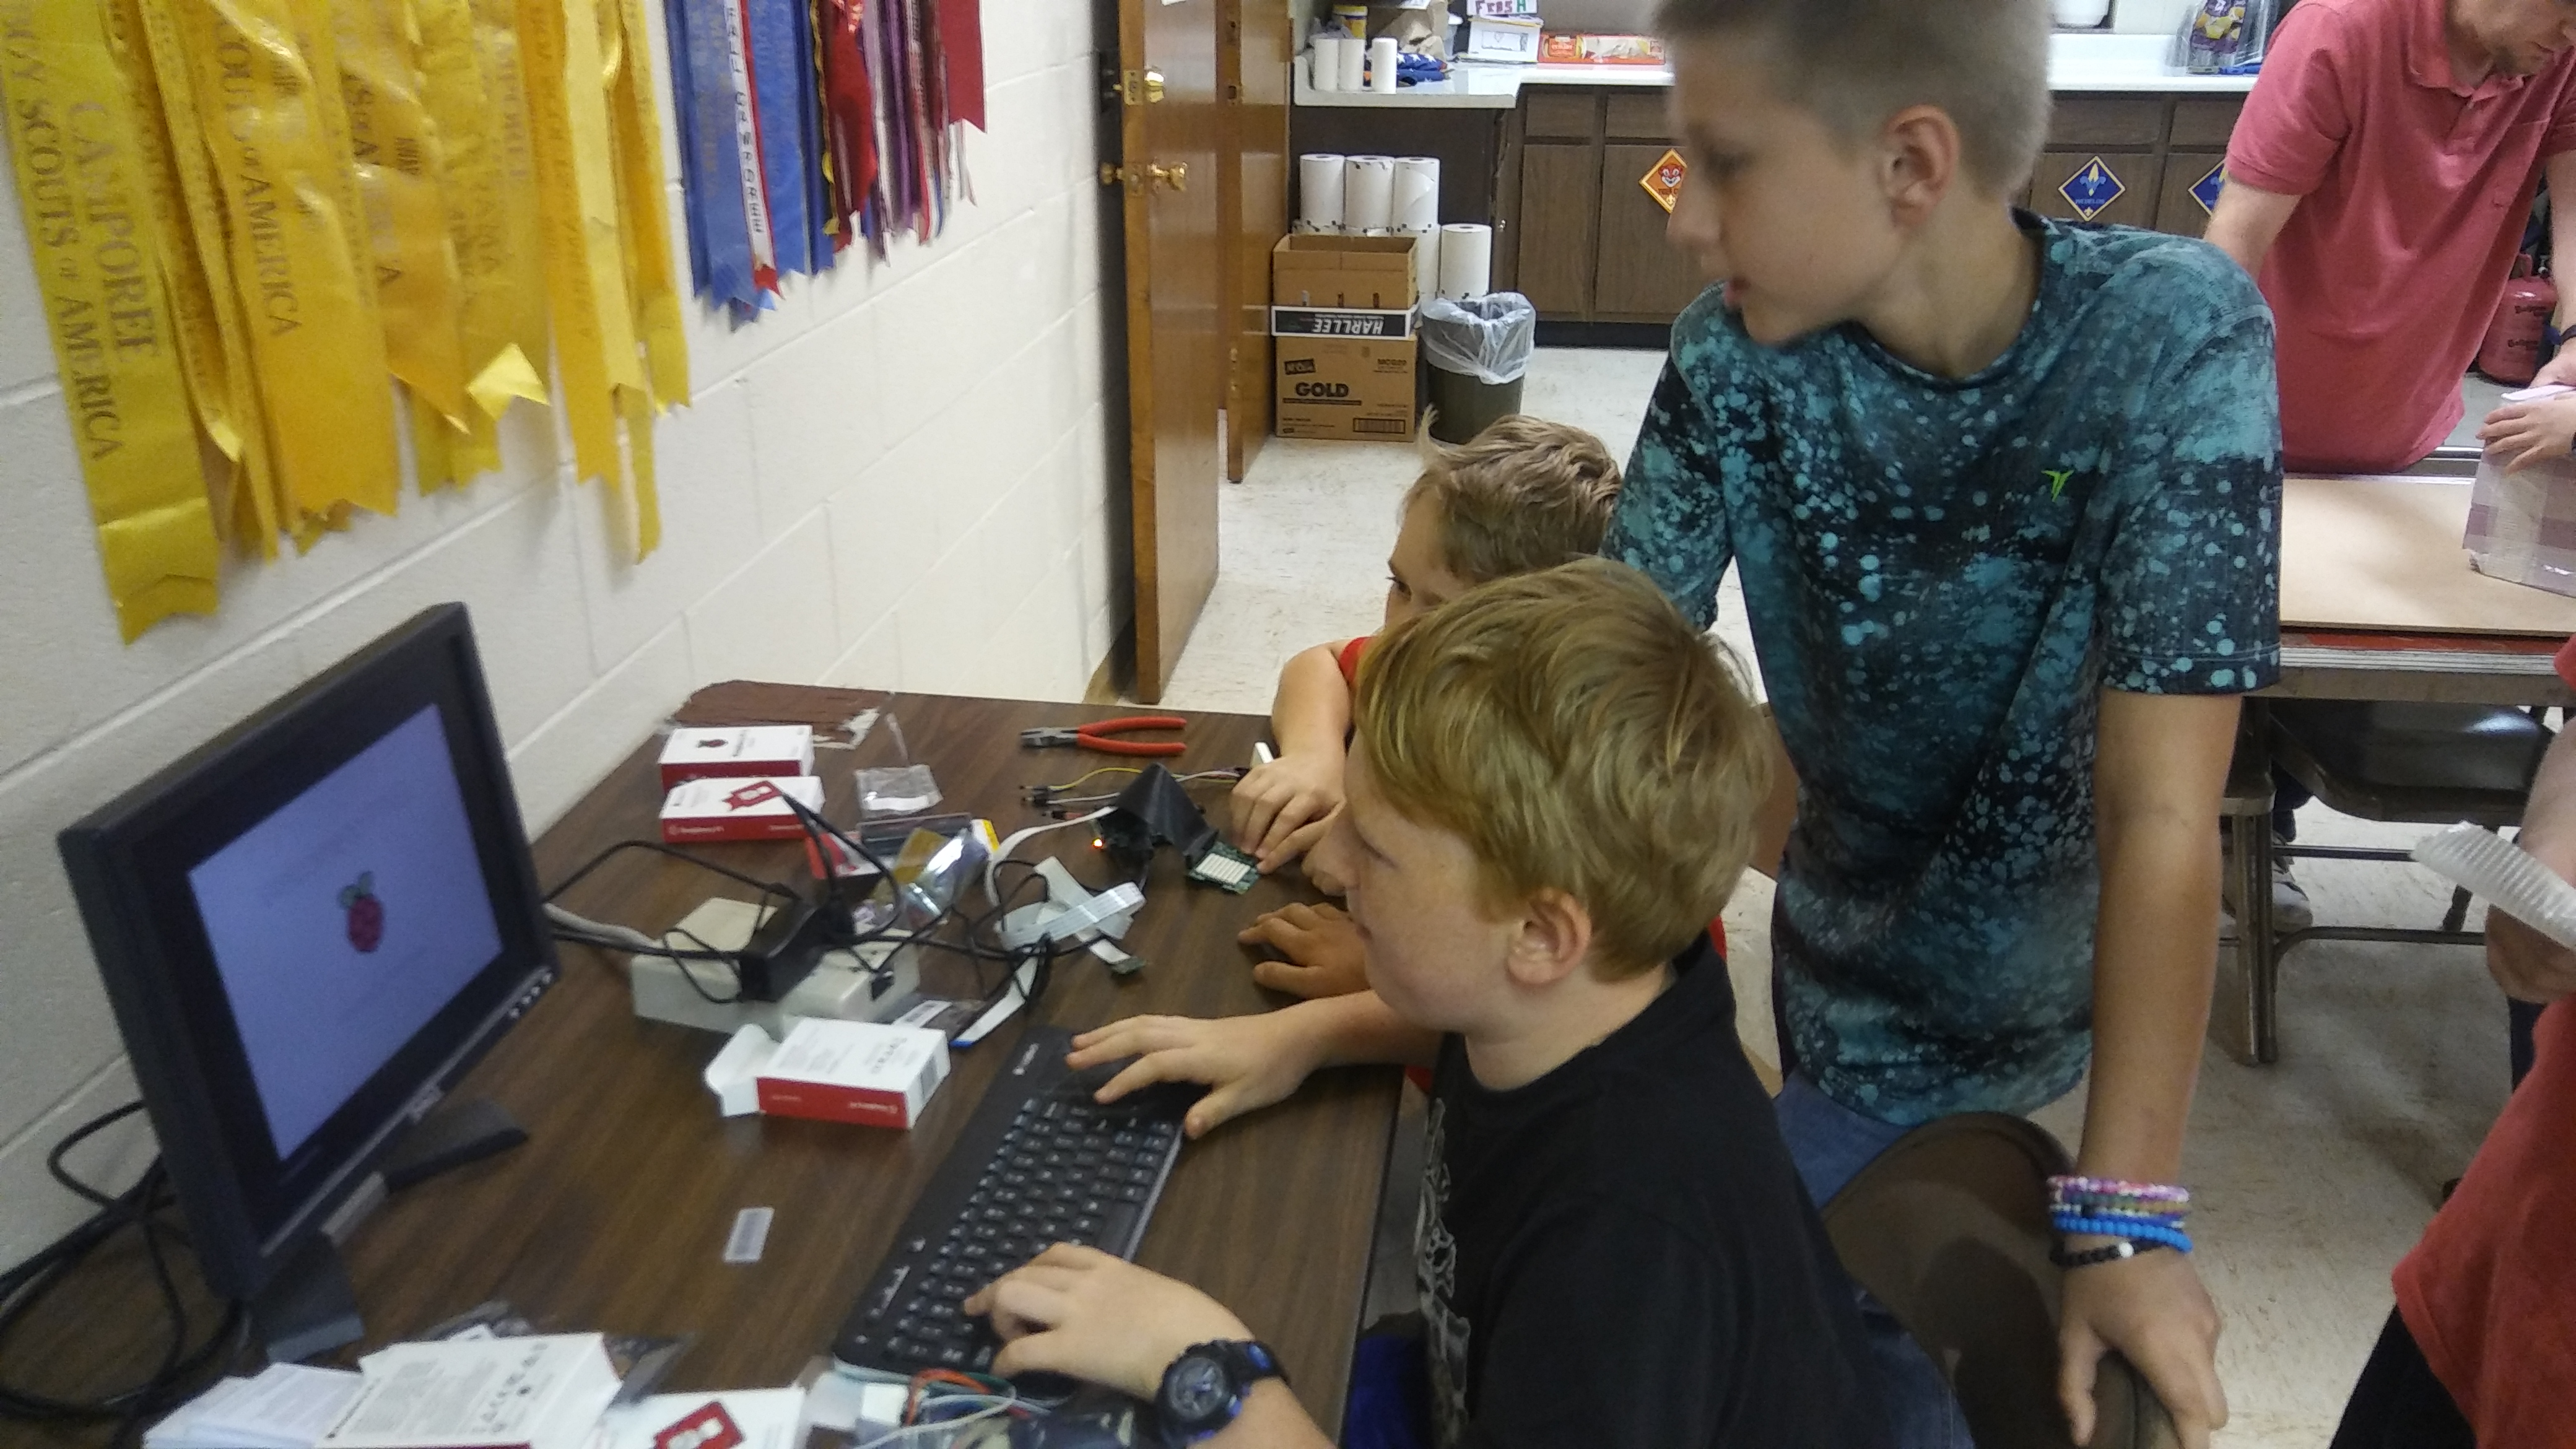
\includegraphics[width=\textwidth]{images/Troop255_Electronics}
    \end{figure}
\end{frame}

\begin{frame}{HabPi 3 - May 13, 2017}
    \begin{figure}
        \centering
        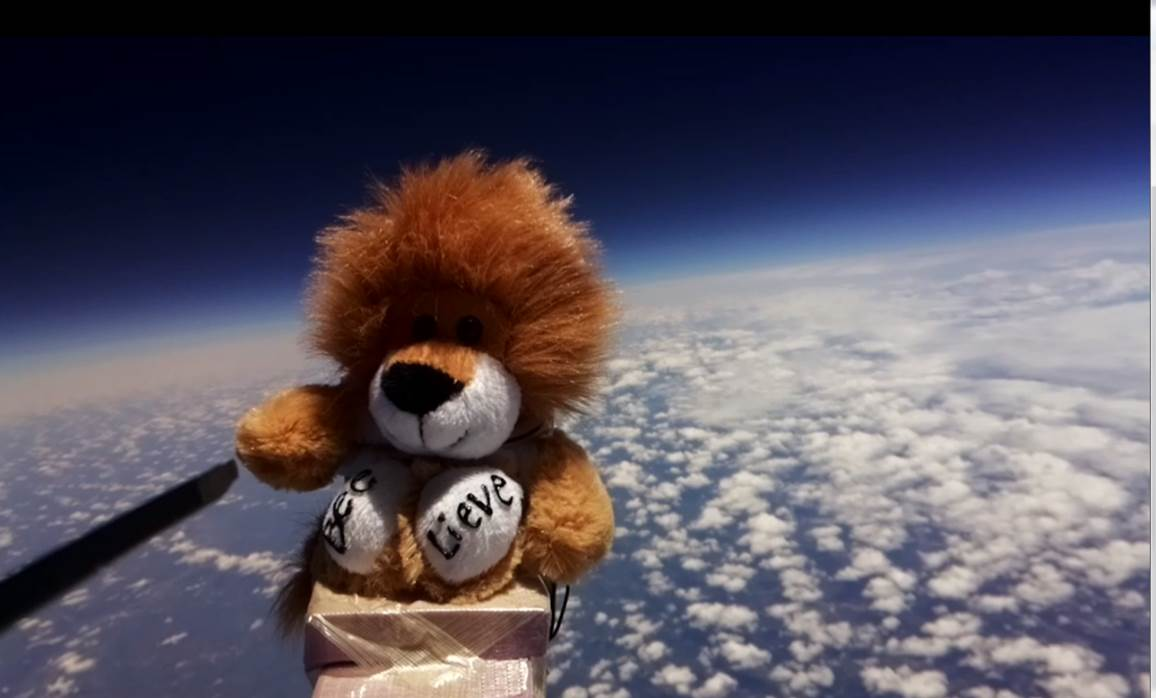
\includegraphics[width=\textwidth]{images/lion}
    \end{figure}
\end{frame}

\begin{frame}{HabPi 4 - July 18, 2017}
    \begin{columns}[t]
        \column{0.5\textwidth}
        \begin{itemize}
            \item Constructed by students in the ARC ORNL Summer Institute
	    \item First HabPi to carry adequate battery power for download
	    \item Released from Pellissippi State Community College
            \item Reached an Altitude of 27,000 Meters 
	    \item Recovered lying neatly beside a farm road
        \end{itemize}

        \column{0.5\textwidth}
        \begin{figure}
            \centering
            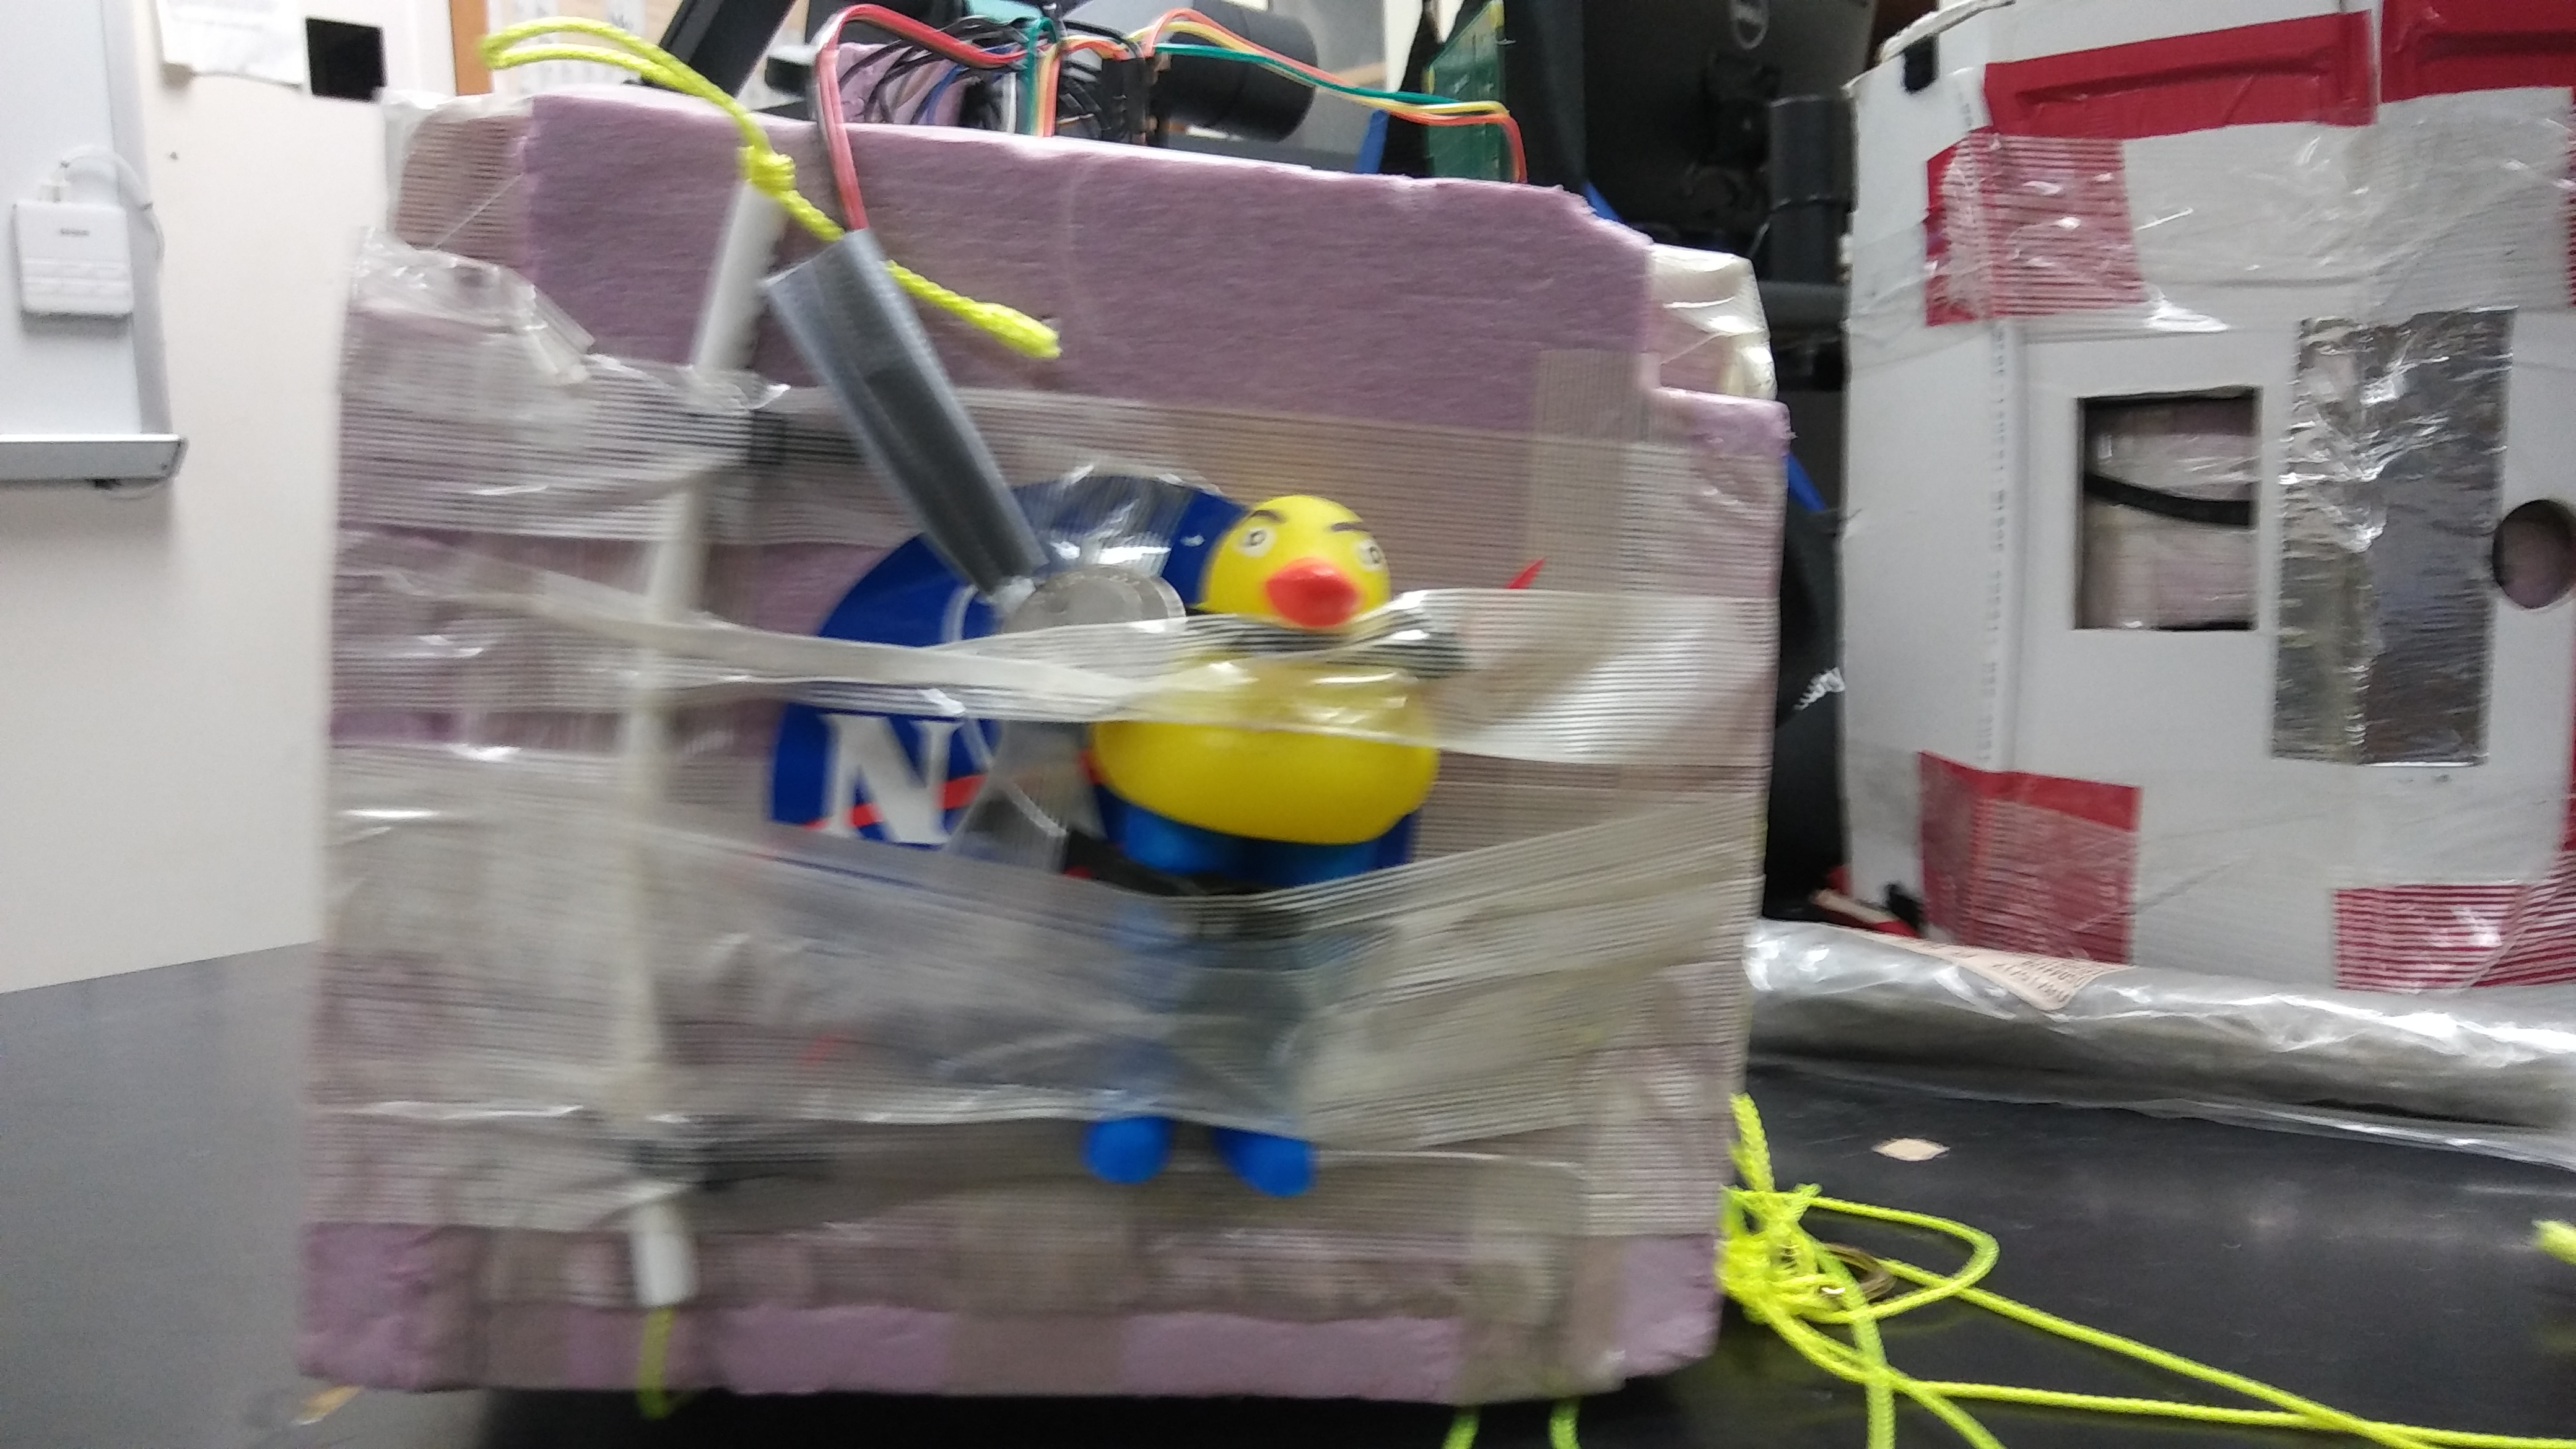
\includegraphics[width=0.75\textwidth]{images/Linda}
            \caption{\tiny Linda}
        \end{figure}
    \end{columns}
\end{frame}

\begin{frame}{HabPi 5 - October 7, 2017}
    \begin{columns}[t]
        \column{0.5\textwidth}
        \begin{itemize}
            \item First flight of a revised HabPi payload
	    \item Released from Athens, TN
            \item Reached an Altitude of 25,000 Meters 
	    \item Recovered from a power line in Knoxville, TN
	    \item Successful test of wireless data download
        \end{itemize}

        \column{0.5\textwidth}
        \begin{figure}
            \centering
            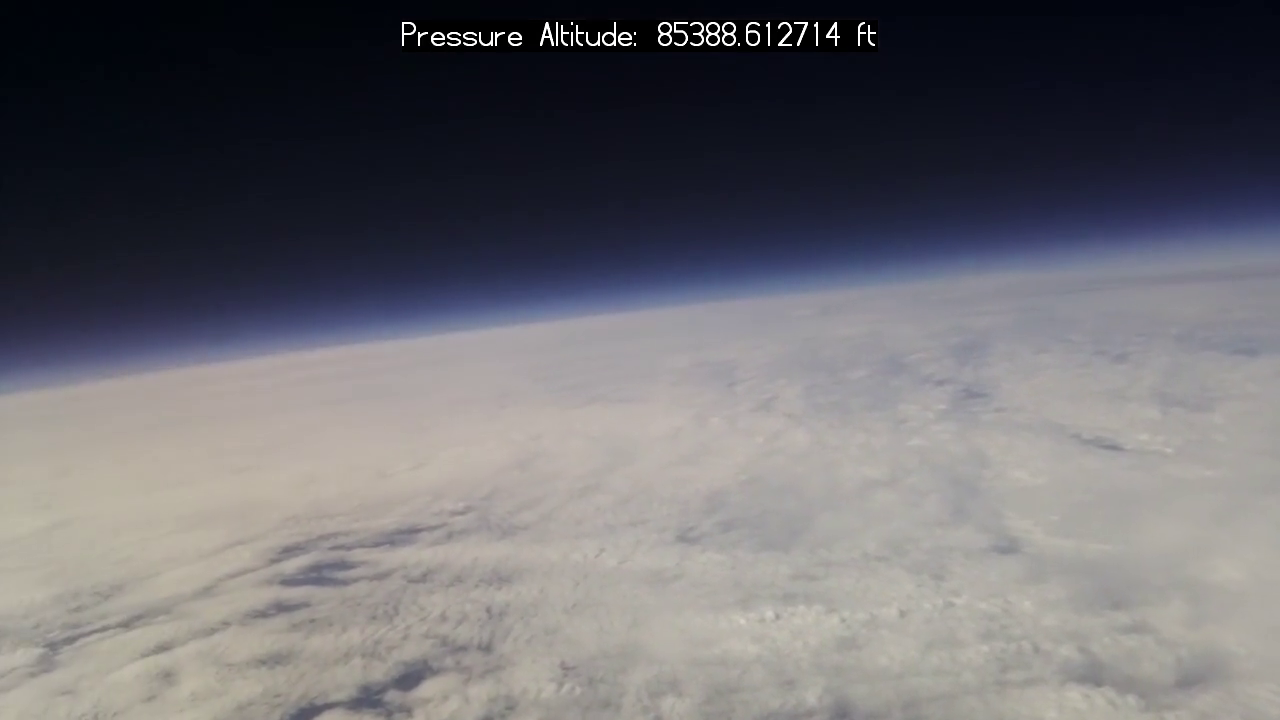
\includegraphics[width=\textwidth]{images/peak-altitude}
            \caption{\tiny HabPi 5 - Peak Altitude}
        \end{figure}
    \end{columns}
\end{frame}

\begin{frame}{Future Directions}
	\begin{columns}
		\column{0.6\textwidth}
		\begin{itemize}
		\item Develop a School Curriculum for HabPi
		\item Improved User Interfaces
		\item A detailed write-up of HabPi construction and flight procedures
		\end{itemize}

		\column{0.4\textwidth}
		\begin{figure}
		\centering
		
\includegraphics[width=\textwidth]{images/habpiGithub}
		\caption{\tiny \tt http://github.com/pngwen/habpi}
		\end{figure}
	\end{columns}
\end{frame}

\begin{frame}[allowframebreaks]{Bibliography}
	\bibliographystyle{plain}
	\bibliography{citations}
\end{frame}

\end{document}


